% ==========================
%  LaTeX 2e - Dokument
%  Editor: Dragan Kozulovic
% ==========================
\documentclass[11pt,a4paper,fleqn]{report}
\usepackage[dvips,final]{graphicx}               %% epsfig 
\usepackage[utf8]{inputenc}                    %% ISO-Text 
\usepackage[T1]{fontenc}                         %% 
\usepackage[german]{babel}                       %% BABEL 
\usepackage{parskip}                             %% 
\usepackage{fancyhdr}                            %% 
\usepackage[hang,bf]{caption}                    %% 
\usepackage{color}                               %% Farben
\usepackage{multirow}                            %% 
%\usepackage{natbib}
\usepackage{float}
\usepackage{siunitx}
\usepackage{textgreek}
\usepackage{amsmath}
\usepackage{graphicx}
\usepackage{subfig}
\usepackage[onehalfspacing]{setspace}
%\usepackage[flushleft]{threeparttable}
\usepackage{blindtext}
\usepackage{amssymb}
%\usepackage{esvect}
%\usepackage[breaklinks]{hyperref} 



% Einzubindende Dateien 
\includeonly{Titelseite,
             Letzte_Seite,
	     eid_erkl,
	     Nomenklatur}
\graphicspath{{./Bilder/}}                         %% Pfad fuer einzubindende Graphiken


% Seiten-Layout
\oddsidemargin   0.0cm                           %% Anpassung DIN A4-Format (symmetrisch)
\evensidemargin  0.0cm                           %% Anpassung DIN A4-Format (symmetrisch)
\topmargin      -1.0cm         
\textheight     25.0cm
\textwidth      16.0cm
\pagestyle{fancy}
\renewcommand{\chaptermark}[1]{\markboth{\thechapter.\ #1}{}}
\renewcommand{\sectionmark}[1]{\markright{\thesection\ #1}}
\fancyhf{}                                %Clears all header and footer fields, in preparation.
\fancyhead[LE,RO]{\thepage}               %Displays the page number in bold in the header,
                                          % to the left on even pages and to the right on odd pages.
\fancyhead[RE]{\nouppercase{\leftmark}}   %Displays the upper-level (chapter) information---
                                          % as determined above---in non-upper case in the header, to the right on even pages.
\fancyhead[LO]{\rightmark}                %Displays the lower-level (section) information---as
                                          % determined above---in the header, to the left on odd pages.
\renewcommand{\headrulewidth}{0.5pt}      %Underlines the header. (Set to 0pt if not required).

%\sloppy                                         %% lockerer Zeilenumbruch
%\flushbottom                                    %% buendige letzte Zeile


% Trennungskorrekturen
%\hyphenation{Bei-spiel}
%\hyphenation{}
%\hyphenation{}
%\hyphenation{}
%\hyphenation{}
%\hyphenation{}


% Umbenennungen (babel) (siehe LaTeX-Begleiter, Abschn. 9.2.3)
\addto\extrasgerman{\renewcommand{\figurename}{Abb.}}


% Listen
\newcommand{\bl}{\begin{list}{\textbullet}%         %% kleine Aufzaehlung/Liste
{\topsep0pt\partopsep0pt\itemsep0pt\parsep0pt\leftmargin1.5em\labelwidth1em\labelsep0.5em}}
\newcommand{\el}{\end{list}}
\newcommand{\cit}[1]{\textit{\cite{#1}}}


% \Literaturverzeichnis
%\usepackage[backend=biber,						% Bibtex-Backend biber mit ACII und Latin 1 Unterst�tzung
%bibencoding=auto,
%natbib=true,									% natbib Zitierbefehle
%bibstyle=numeric,								% Numerisches Literaturverzeichnis
%giveninits=true,								% Vor- und Mittelnamen als Initialien
%citestyle=numeric,								% Numrische Zitierweise
%url=false,										% Schreibe nicht die URL ins %Literaturverzeichnis
%maxbibnames=3,									% Maximal 3 Autoren im Literaturverteichnis
%minbibnames=3									% Maximal 3 Autoren im %Literaturverteichnis
%]{biblatex}


%\DeclareNameAlias{default}{last-first}			% Nachname, Vorname in Literaturverzeichnis
%\renewcommand{\labelnamepunct}{\addcolon\space}	% Doppelpunkt nach Autoren vor Titel
%\renewbibmacro*{journal+issuetitle}{			% number in Klammern
%  \usebibmacro{journal}%
%  \setunit*{\addspace}%
%  \iffieldundef{series}
%    {}
%    {\newunit
%     \printfield{series}%
%     \setunit{\addspace}}%
 % \printfield{volume}%
%  \iffieldundef{number}
 %    {}
%      {\mkbibparens{\printfield{number}}}%
%  \setunit{\addcomma\space}%
%  \printfield{eid}%
%  \setunit{\addspace}%
%  \usebibmacro{issue+date}%
%  \setunit{\addcolon\space}%
%  \usebibmacro{issue}%
%  \newunit}

\usepackage{calc}								% Arithmetische Latex-Befehle





\begin{document}
% Titelseite
\begin{titlepage}
 \centering

\begin{table}[htbp]
 \begin{center}
 \vspace{-0.5cm}
% \renewcommand{\arraystretch}{1.5}
  \begin{tabular}{lcr} 
    \parbox{0.45\textwidth}{\mbox{ }} & \parbox{0.13\textwidth}{\mbox{ }} & \parbox{0.45\textwidth}{\mbox{ }} \\
    \hspace*{-2.0cm}
    
\includegraphics[width=0.5\textwidth]{./Bilder/TUBraunschweig_4C.pdf} &		 					\includegraphics*[width=0.6\textwidth]{./Bilder/ifw_logo.png} 
       \\ %empty
  \end{tabular}
 \end{center}
\end{table}


 \vspace*{2.0cm}

 \textbf{\large Projektarbeit WS 2019/2020}


 \vspace*{1.5cm}
 
 \textbf{\LARGE  Maximierung der Zugfestigkeit einer Verdichterschaufel aus der Titanlegierung Ti-6Al-2Sn-4Zr-2Mo} \\[0.5ex]


 \vspace*{1.5cm}

 \textbf{\large Ziad Ben Hadj Salem} \\[0.5ex]
 \textbf{Matrikelnummer 4880262}
 
 \textbf{\large Thiago Coelho Jordao} \\[0.5ex]
 \textbf{Matrikelnummer 4898717}
 
 \textbf{\large Patrick Hartmann} \\[0.5ex]
 \textbf{Matrikelnummer 4880903}

 \textbf{\large Viktor Rein} \\[0.5ex]
 \textbf{Matrikelnummer 4808590}
 

 

 



 \vspace*{2.5cm}

 \begin{table}[htbp]
  \begin{center}
%  \renewcommand{\arraystretch}{1.5}
   \begin{tabular}{rl} 
     \parbox{0.33\textwidth}{\mbox{ }} & \parbox{0.66\textwidth}{\mbox{ }} \\
     Ausgegeben: & Institut für Werkstoffe \\
                 & Institutsleiter: Prof. Dr. Joachim Rösler \\
                 & Technische Universit\"at Braunschweig \\
                 &  \\
       Betreuer: & Carsten Siemers\\
       			 & Fabian Haase\\
 %(Erstellt bei:) & (Externe Firma, Stadt) \\
                 %&  \\
 Prüfer: & Priv.~-Doz.~Dr. M. Bäker \\
   \end{tabular}
  \end{center}
 \end{table}



\end{titlepage}


%only blank page
\newpage
\thispagestyle{empty}
\mbox{}


\pagenumbering{roman}\setcounter{page}{1} 


%% Eidesstattliche Erklaerung (fuer DA, MA und BA)
\chapter*{Eidesstattliche Erkl"arung}\label{s:eid_erkl}


Hiermit erklären wir, Ziad Ben Hadj Salem, Thiago Coelho Jordao, Patrick Hartmann und Viktor Rein des Eides statt, die vorliegende Projektarbeit selbstständig und ohne
fremde Hilfe verfasst und keine anderen als die angegebenen Hilfsmittel verwendet zu
haben.

\vspace*{3cm}
Braunschweig, Datum




% Uebersicht
%\include{abstract}
%\include{empty_page}


% Inhaltsverzeichnis
\fancyhead[RE]{Inhaltsverzeichnis}
\fancyhead[LO]{Inhaltsverzeichnis}
{ 
   \renewcommand{\baselinestretch}{0.85}    %% Zeilenabstand / TOC
   \small\normalsize                        %% neuen Zeilenabstand aktivieren
   \tableofcontents
}
% ATTENTION: comment out if contents sides are even number
%\include{empty_page}


% Nomenklatur
\newpage
\fancyhead[RE]{Nomenklatur}
\fancyhead[LO]{Nomenklatur}
\chapter*{Nomenklatur}
\addcontentsline{toc}{chapter}{Nomenklatur}



\subsection*{Formelzeichen}
\begin{tabbing}
	\hspace*{2cm}\=\kill
	$R_m$ \> Zugfestigkeit \\[0.2ex]
	$R_{p0,2}$ \> Dehngrenze mit 0,2\% plastischer Verformung \\[0.2ex]
	$A$ \> Bruchdehnung \\[0.2ex]
	$S_0$ \> Anfangsquerschnittsfläche \\[0.2ex]
	$l_0$ \> Anfangslänge \\[0.2ex]
	$E$ \> Elastizitätsmodul \\[0.2ex]
	$A_g$ \> Gleichmaßdehnung \\[0.2ex]
	$HV$ \> Vickershärte \\[0.2ex]
	$\Delta l$ \> Längenänderung \\[0.2ex]
	
\end{tabbing}

\subsection*{Griechische Bezeichnungen}
\begin{tabbing}
	$\epsilon$ \> Dehnung \\[0.2ex]
	$\sigma$ \> Spannung \\[0.2ex]
	
\end{tabbing}




\begin{table}[] 
	\centering 
	\begin{tabular}{lr} 
		
		Name & \hspace{0.5cm} Initialen\\ 
		\hline 
		Ziad Ben Hadj Salem & ZB\\
		Thiago Coelho Jordao & TJ\\
		Patrick Hartmann & PH\\
		Viktor Rein & VR\\
		\hline
		
	\end{tabular} 
	\caption{Initialen der beteiligten Personen} 
	\label{tab:initialien} 
\end{table} 




% alle Kapitel
\pagenumbering{arabic}\setcounter{page}{1}
\fancyhead[RE]{\nouppercase{\leftmark}}
\fancyhead[LO]{\rightmark}

\chapter{Einleitung} 
Titan nimmt durch seine herausragenden Eigenschaften eine immer stärkere Rolle im Bereich der Luft- und Raumfahrttechnik ein. Dazu zählen Eigenschaften wie die hohe spezifische Festigkeit, Korrosions- und Temperaturbeständigkeit sowie die Dauerfestigkeit, Kriechbeständigkeit und Rissausbreitung. Diese sind abhängig von der Mikrostruktur des Werkstoffs, die maßgeblich durch die Legierungszusammensetzung und thermomechanische Behandlung bestimmt wird. Dadurch wird eine Vielzahl an Anwendungen in verschiedensten Bereichen des Flugzeugbaus, wie der Flugzeugzelle, dem Fahrwerk und den Triebwerken ermöglicht. Trotz der durch den großen Produktionsaufwand relativ hohen Werkstoffkosten hat sich Titan durch die vorteilhafte Kombination seiner Eigenschaften in der militärischen und zivilen Luftfahrt durchgesetzt. \\ 
%Die Möglichkeit durch die Mikrostruktur die Eigenschaften des Titans bedarfsgerecht einzustellen ist der allotropen Phasenumwandlung bei $882\circ C$ von einem kubisch-raumzentrierten (krz) Gitter ($\beta$-Phase) zu einer hexagonal annähernd dichtesten Packung (hdp) ($\alpha$-Phase) bei Raumtemperatur geschuldet. Dabei kann durch Zugabe von Legierungselementen die Übergangstemperatur der allotropen Umwandlung abgesenkt ($\beta$-stabilisierend) oder angehoben werden ($\alpha$-stabilisierend). Die hier betrachtete Legierung Ti 6Al 2Sn 4Zr 2Mo (Ti6242) hat durch den $\beta$-isomorphen Stabilisator Molybdän eine eine geringere $\beta$-Transus-Temperatur mit steigendem Molybdänanteil, sodass die $\beta$-Phase auch bei Raumtemperatur stabil sein kann. %

Die gängigste Wärmebehandlung für Ti6242 ist ein Glühen im Zweiphasenfeld knapp unter der $\beta$-Transus-Temperatur und anschließendes Abkühlen an der Luft. Dadurch entsteht ein bimodales Gefüge bestehend aus Primär-$\alpha$-Körnern ($\alpha_p$) und lamellaren transformierten $\beta$-Körnern. 

Ein Großteil der in der Luftfahrt eingesetzten Titanlegierungen bestehen aus zwei Phasen, der $\alpha$ und $\beta$-Phase in unterschiedlichen Volumenanteilen und Morphologien. Die bekannteste und am besten erforschte Legierung ist dabei Ti 6Al 4V (Ti64), an der bereits seit den 50er Jahren geforscht wird. Ti64 wird insbesondere in dynamisch belasteten Bauteilen wie Fanschaufeln in Flugtriebwerken und Verbindungselementen wie Nieten und Bolzen. 

Ziel dieser Projektarbeit ist die Zugfestigkeit der Legierung Ti6242 durch eine Wärmebehandlung zu maximieren, während eine Bruchdehnung von mindestens 10\% beibehalten wird.  

\begin{table}[h] 
	\centering 
	\begin{tabular}{lr} 
		
		Name & \hspace{0.5cm} Initialen\\ 
		\hline 
		Ziad Ben Hadj Salem & ZB\\
		Thiago Coelho Jordao & TJ\\
		Patrick Hartmann & PH\\
		Viktor Rein & VR\\
		\hline
		
	\end{tabular} 
	\caption{Initialen der beteiligten Personen} 
	\label{tab:initialien} 
\end{table} 

\chapter{Metallurgie}	

\section{Metallurgie von Titan und Titanlegierungen (PH)}
Reines Titan ist das vierthäufigste Metall in der Erdkruste (etwa 0,4 -- 0,6 \%) und zeigt eine hohe Reaktivität mit anderen Elementen des Periodensystems. Es tritt in zwei verschiedenen Gittermodifikationen auf. Es gibt die $\alpha$-Phase, die ein hexagonales Gitter annähernd dichtester Kugelpackung (hex) aufweist. Außerdem gibt es die $\beta$-Phase, die eine kubisch-raumzentrierte Gitterstruktur (krz) besitzt (Abbildung \ref{fig:Kristallgitter}). Bei einer Temperatur von $882 \pm 2 ^\circ C$ tritt eine Phasenumwandlung von $\alpha$ zu $\beta$ auf. Die Temperatur, bei der diese Umwandlung stattfindet, ist eine wichtige Kenngröße im Bereich der Titanwerkstoffe und wird $\beta$-Transus-Temperatur ($T_{\beta}$) genannt.
Die Umwandlung $\beta$ zu $\alpha$ kann durch einen diffusionskontrollierten Keimbildungs- und Wachstumsprozess oder durch einen diffusionslosen Umklappvorgang (martensitisch) erfolgen, wenn eine ausreichend schnelle Abkühlgeschwindigkeit (über 500 K/s) erzielt wird \cite{C.Leyens.2005,Lutjering.2007}.

\begin{figure}[h]
	\centering
	\subfloat{}
	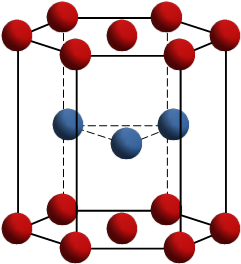
\includegraphics[width=0.3\textwidth]{./Bilder/hcp}
	\hspace{4ex}
	\subfloat{}
	\includegraphics[width=0.3\textwidth]{Bilder/krz}
	\caption{Kristallgitterstruktur der $\alpha$-Phase (hex) und $\beta$-Phase (krz)}
	\label{fig:Kristallgitter}
\end{figure}

\subsection{Klassifizierung von Titan und Titanlegierungen}

Da reines Titan wie alle anderen Metalle keine hohe Festigkeit besitzt, werden Legierungen hergestellt, um die mechanischen Eigenschaften gezielt zu verändern. Die in der Industrie erhältlichen Titanlegierungen werden daher in verschiedene Klassen eingeteilt. Es gibt technisch reines Titan (CP-Titanium), $\alpha$-, $\alpha+\beta$-, metastabile $\beta$- sowie die $\beta$-Legierungen. Die $\alpha+\beta$-Legierungen werden zusätzlich in near-$\alpha$- und near-$\beta$-Legierungen aufgeteilt. Für die Klassifikation ist der Anteil an $\beta$-Phase im Gefüge bei Raumtemperatur entscheidend.
Die für Titanwerkstoffe typischen Legierungselemente werden in vier Kategorien eingeteilt, die sich in ihrer Wirkungsweise unterscheiden. 
Als $\alpha$-Stabilisatoren werden Legierungselemente wie Aluminium (Al), Sauerstoff (O) und Stickstoff (N) bezeichnet, die zu einer Einschnürung des $\beta$-Phasengebietes führen und die $\beta$-Transus-Temperatur erhöhen.
Des Weiteren gibt es die $\beta$-Stabilisatoren, die das $\beta$-Phasengebiet erweitern und die $\beta$-Transus-Temperatur verringern. Man unterscheidet bei den $\beta$-Stabilisatoren zwischen $\beta$-isomorphen und $\beta$-eutektoiden Stabilisatoren. Zu den $\beta$-isomorph wirkenden Stabilisatoren gehören die Elemente Molybdän (Mo), Vanadium (V), Niob (Nb) und Tantal (Ta). Diese erweitern das $\beta$-Phasengebiet bis zur Raumtemperatur. 
Zu den $\beta$-eutektoiden-Stabilisatoren gehören Elemente wie Eisen (Fe), Chrom (Cr), Kupfer (Cu), Mangan (Mn) und Silizium (Si). Bei diesen Stabilisatoren kommt es unterhalb einer elementabhängigen Grenztemperatur zu einer eutektoiden Reaktion, die zu einer Ausscheidung einer zusätzlichen Phase führt. Die Elemente Zinn (Sn) und Zirkon (Zr) werden häufig als neutral bezeichnet, da diese nur eine sehr geringe $\alpha$-stabilisierende Wirkung haben. Einen Überblick über den Einfluss der Legierungselemente auf $\alpha$- und $\beta$-Phase gibt die Abbildung \ref{fig:tabelle-1}.

\begin{figure}[h]
	\centering
	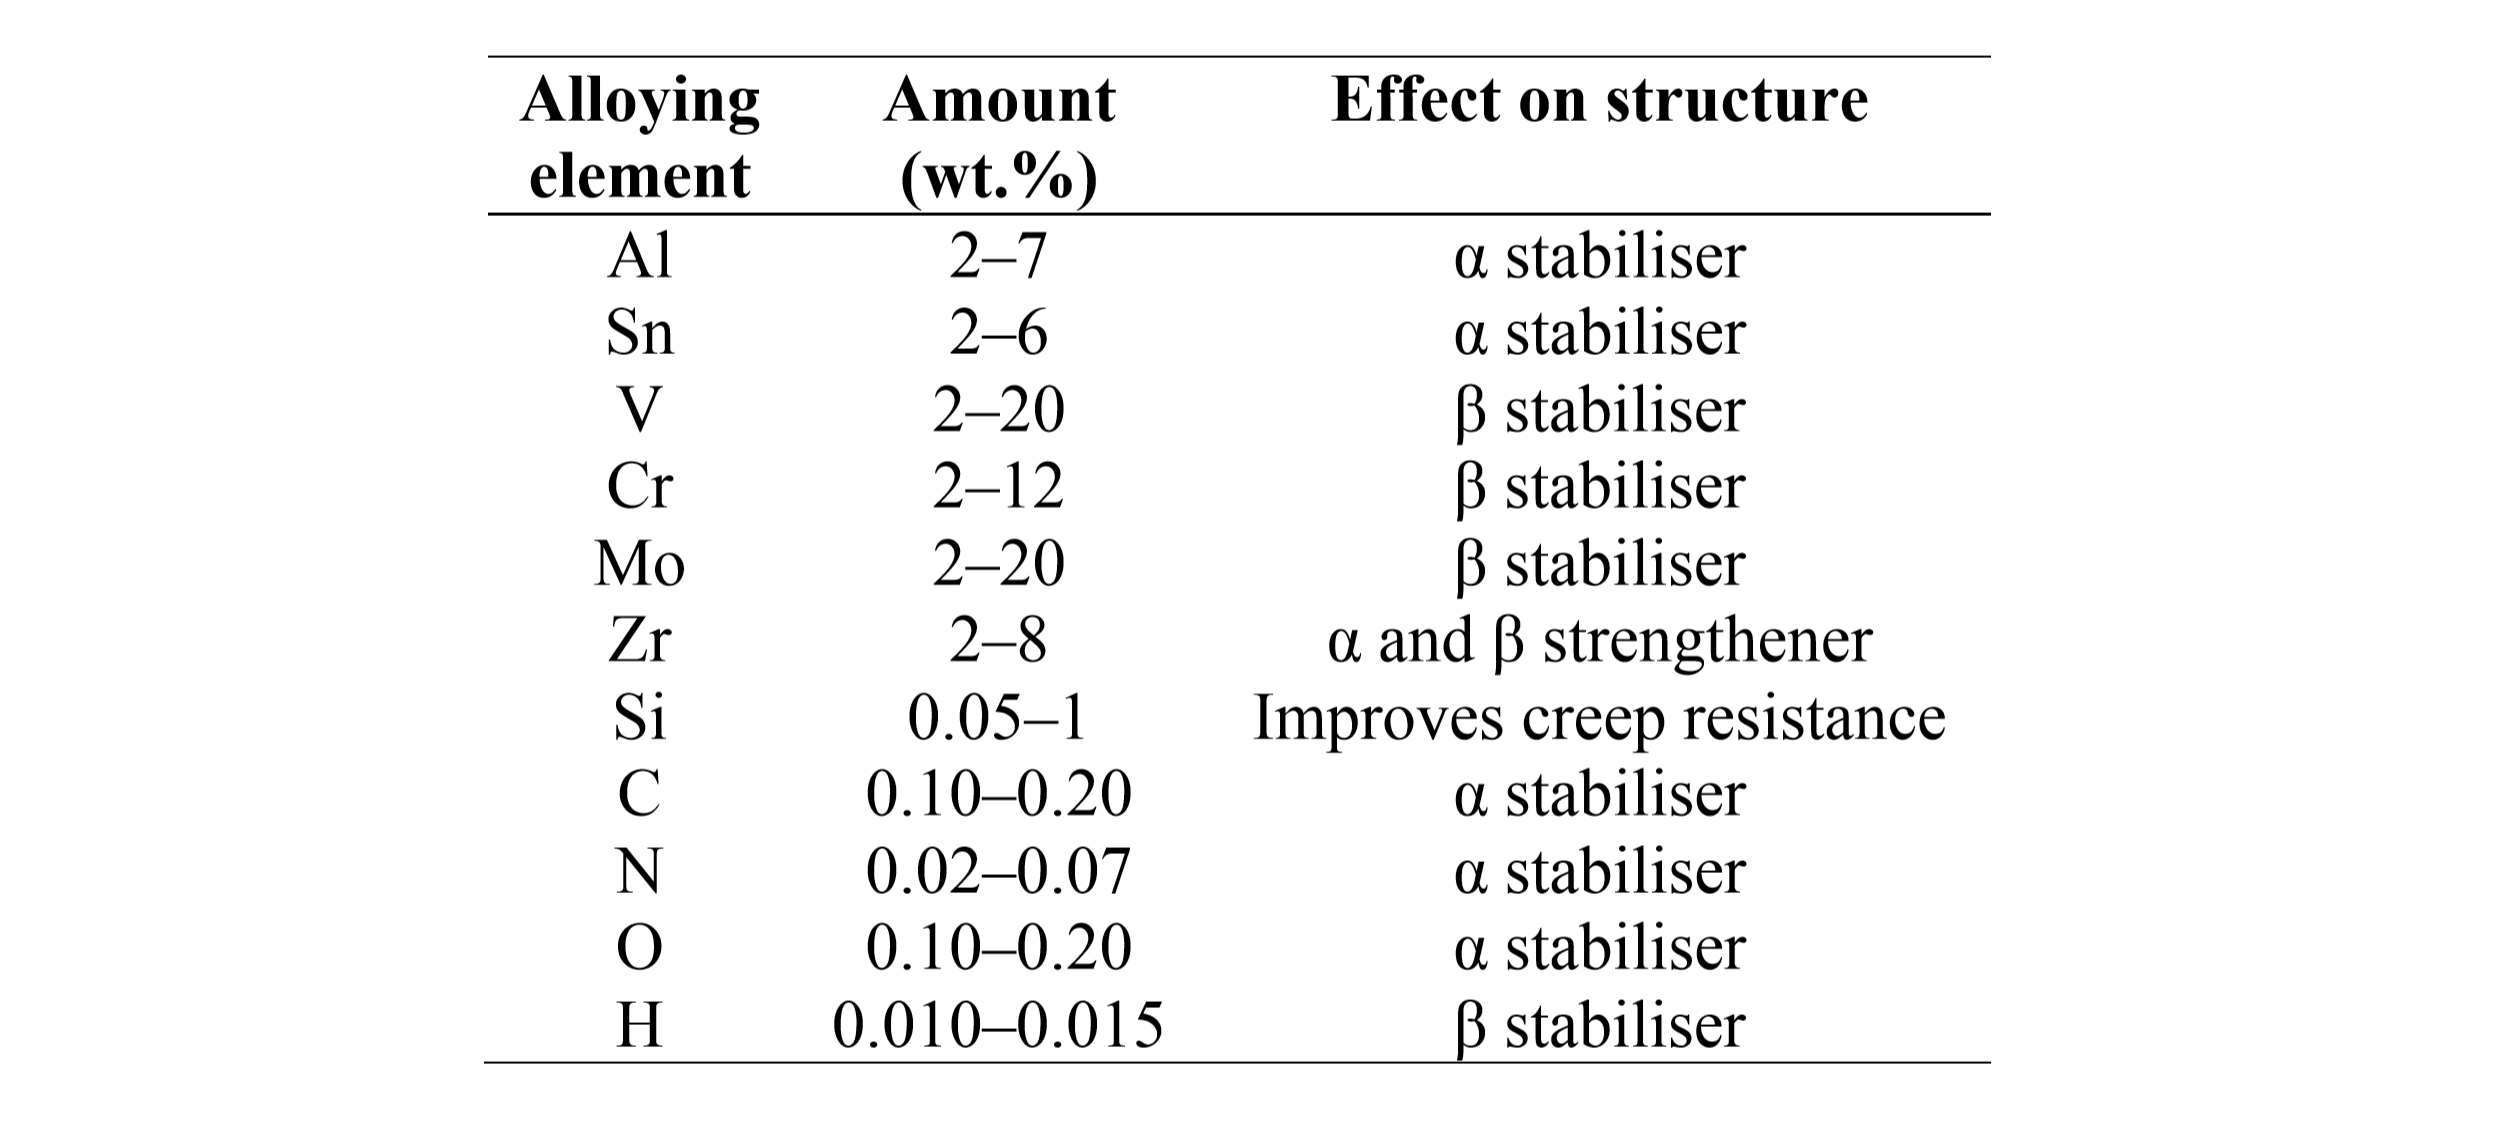
\includegraphics[width=0.9\linewidth]{./Bilder/Tabelle 1.png}
	\caption{Einfluss der Legierungselemente auf $\alpha$- und $\beta$-Phase (schematisch) \cite{Lutjering.2007}}
	\label{fig:tabelle-1}
\end{figure}

Bei einer Wärmebehandlung von near-$\alpha$-, $\alpha$+$\beta$- oder metastabilen $\beta$-Titanlegierungen im Zweiphasengebiet (also unterhalb der $\beta$-Transus-Temperatur) kommt es bei ausreichend langen Glühzeiten zum sogenannten Element Partitioning \cite{Lutjering.2007}. Dabei diffundieren die $\alpha$-stabilisierenden Elemente in die $\alpha$-Phase und die $\beta$-stabilisierenden Elemente in die $\beta$-Phase, sodass die lokale chemische Zusammensetzung der jeweiligen Phasen von der globalen chemischen Zusammensetzung einer Legierung abweichen kann.



\paragraph{CP-Titanium} 
Technisch reines Titan (\textit{commercially pure}, CP) enthält nur Sauerstoff und Eisen als zusätzliche Legierungselemente, jedoch sind Begleitelemente/Verunreinigungen in bestimmten Mengen zugelassen und auch nicht zu vermeiden. In welche Klasse technisch reines Titan eingeordnet wird, hängt von der chemischen Zusammensetzung ab. Es gibt 4 Klassen, die sogenannten CP-Grades \cite{C.Leyens.2005}.

\paragraph{$\alpha$- und near-$\alpha$-Legierungen}
Werden $\alpha$-Stabilisatoren dem reinen Titan hinzulegiert, führt dies zu den sogenannten $\alpha$-Legierungen. Wird ein kleiner Anteil an $\beta$-Stabilisatoren ( 1--2 Gew.\%) hinzugefügt, führt dies zu einer near-$\alpha$-Legierung mit einem kleinen Anteil an $\beta$-Phase (\textless5\%) bei Raumtemperatur. Ein typisches Beispiel einer $\alpha$-Legierung ist Ti–5Al–2.5Sn. Zu den Vertretern von near-$\alpha$-Legierungen gehören Ti–8Al–1Mo–1V und Ti–6Al–2Sn–4Zr–2Mo. Der Aluminiumgehalt in diesen Legierungen wird typischerweise unter 9\% gehalten, da es sonst zu Ti$_3$Al-Ausscheidungen und dadurch zu Versprödungen kommen kann \cite{C.Leyens.2005,Lutjering.2007,Boyer.2007,M.J.Donachie.2010}.

\paragraph{$\alpha$+$\beta$-Legierungen}
Diese Legierungen bilden die erste Untergruppe der zweiphasigen Titanlegierungen. Bei Raumtemperatur besitzen sie zwischen 5\% und 35\% $\beta$-Phase im Gefüge. Sie können dabei vollständig oder teilweise martensitsch ($\alpha'$- oder $\alpha''$-Phase) umwandeln. Die bekanntesten $\alpha$+$\beta$-Legierungen sind Ti–6Al–4V und Ti–6Al–2Sn–4Zr–6Mo \cite{C.Leyens.2005,Lutjering.2007,Boyer.2007,M.J.Donachie.2010}.

Die metastabilen $\beta$-, near-$\beta$- und $\beta$-Legierungen werden an dieser Stelle nicht näher erläutert, da sie für diese Arbeit nicht relevant sind.

\subsection{Mikrostrukturen in Titanlegierungen}
Im Bereich der Titanlegierungen gibt es drei Basis-Mikrostrukturen, die eingestellt werden können. Es gibt lamellare, globulare und Bi-modal/Duplex-Gefüge \cite{C.Leyens.2005,Lutjering.2007,Boyer.2007,M.J.Donachie.2010}.

Mikrostrukturen, die man während des Gießens erhält, sind sehr grob und besitzen eine geringe Festigkeit. Daher werden diese Mikrostrukturen mithilfe von thermo-mechanischen Prozessschritten geziehlt modifiziert. Dazu gehören die Verfeinerung der Mikrostruktur durch Rekristallisation oder die Formation neuer Mikrostrukturen durch Kornwachstum \cite{C.Leyens.2005,Lutjering.2007,Boyer.2007,M.J.Donachie.2010}.

Typische thermo-mechanische Prozessschritte für Near-$\alpha$- und $\alpha+\beta$-Legierungen beinhalten die Homogenisierung (solution heat treatment), Deformation, Rekristallisation, das Altern (ageing) und Spannungsarmglühen (stress relief annealing). Die $\beta$-Transus-Temperatur spielt dabei eine entscheidende Rolle, welche Gefüge sich bei den Legierungen einstellen \cite{C.Leyens.2005,Lutjering.2007,Boyer.2007}.
 
Eine kurze Beschreibung dieser Mikrostrukturen ist im folgenden aufgeführt.

\begin{itemize} 
	\item lamellare Mikrostruktur: Das Glühen und Abschrecken oberhalb der $\beta$-Transus-Temperatur führt zu einer vollständigen martensitischen Umwandlung. Das entstandene Gefüge liegt dann metastabil in der $\alpha'$-Phase vor. Ein Beispiel für diese lamellare Mikrostruktur zeigt Abbildung \ref{fig:abbildung-3}. Bei einer langsamen Abkühlung von oberhalb der $\beta$-Transus-Temperatur stellt sich ein sogenanntes Widmannstättengefüge ein. So bilden sich beim Unterschreiten der $\beta$-Transus-Temperatur an bevorzugten Stellen $\alpha$-Keime, die in die $\beta$-Körner hineinwachsen. Aufgrund von Orientierungsbeziehungen zwischen $\alpha$- und $\beta$-Phase wachsen die $\alpha$-Körner in eine Vorzugsrichtung. Dadurch ensteht ein lamellares Gefüge, dass aus $\alpha$-Lamellen besteht und von schmalen Bereichen von $\beta$-Phase umschlossen ist.
	
\item globulare Mikrostruktur: Bei einer abschließenden Wärmebehandlung im Zweiphasengebiet mit tiefen Temperaturen ist der Anteil an Primär-$\alpha$ im Gefüge höher. Diese globularen $\alpha$-Körner werden dann nur von einem schmalen Rand von $\beta$-Phase umschlossen \cite{Lutjering.2007}. Abbildung \ref{fig:abbildung-5} zeigt ein Beispiel eines globularen Gefüges.

\item bi-modale Mikrostruktur: Das bi-modale oder Duplex-Gefüge entsteht, wenn knapp unterhalb der $\beta$-Transus-Temperatur geglüht und anschließend an der Luft abgekühlt wird. Beim Glühen in diesem Temperaturbereich besteht das Gefüge aus globularem $\alpha$- und $\beta$-Körnern. Beim abkühlen wandeln die $\alpha$-Körner nicht mehr um, da sie sich bereits in der $\alpha$-Phase befinden, die bei tiefen Temperaturen beständig ist. Diese werden daher als Primär-$\alpha$ oder $\alpha_p$ bezeichnet. Aus der $\beta$-Phase scheidet sich beim Abkühlen $\alpha$-Phase in Form von Lamellen aus. Man spricht dann von transformierten $\beta$. Bereiche, in denen Lamellen dicht beieinander liegen mit gleicher Orientierungsrichtung nennt man $\alpha$-Lamellenpakete \cite{Lutjering.2007}. Abbildung \ref{fig:abbildung-4} zeigt ein bi-modales Gefüge von Ti-6242. 

\begin{figure}[h]
	\centering
	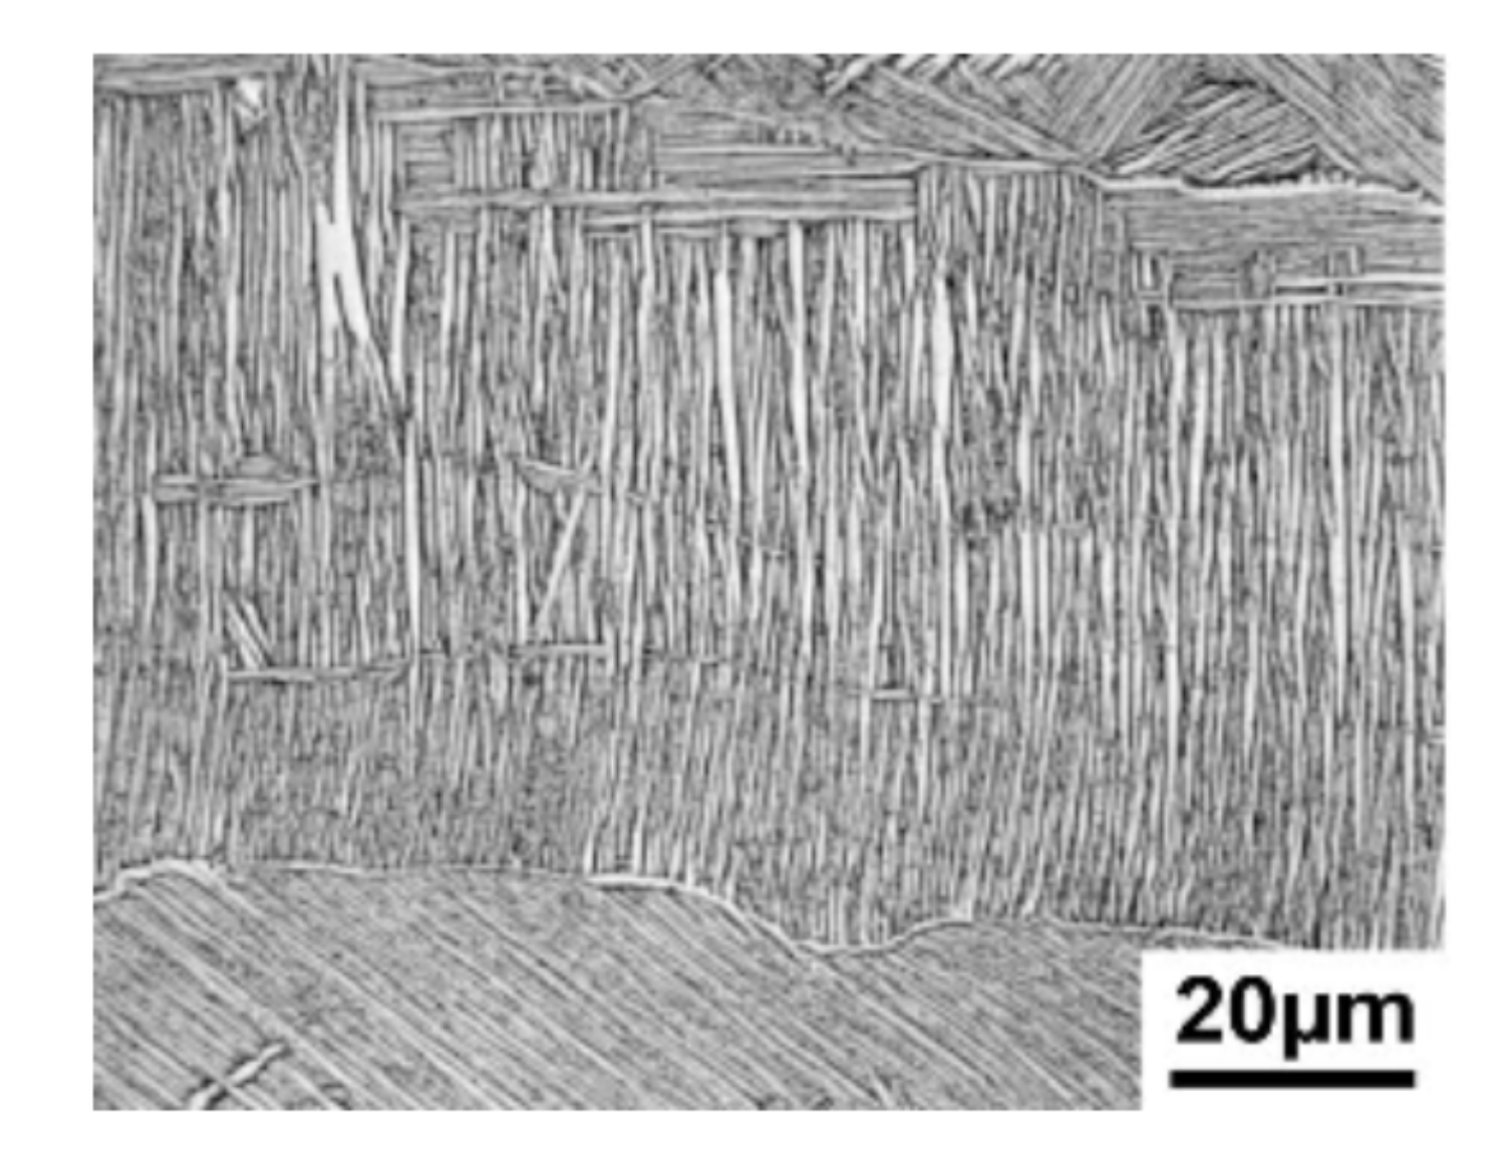
\includegraphics[width=0.7\linewidth]{./Bilder/Abbildung 3.png}
	\caption[Abbildung 3]{lamellare Mikrostruktur von Ti-6242, Abkühlrate ca 100$^\circ$C/min \cite{Lutjering.2007}}
	\label{fig:abbildung-3}
\end{figure}

\begin{figure}[h]
	\centering
	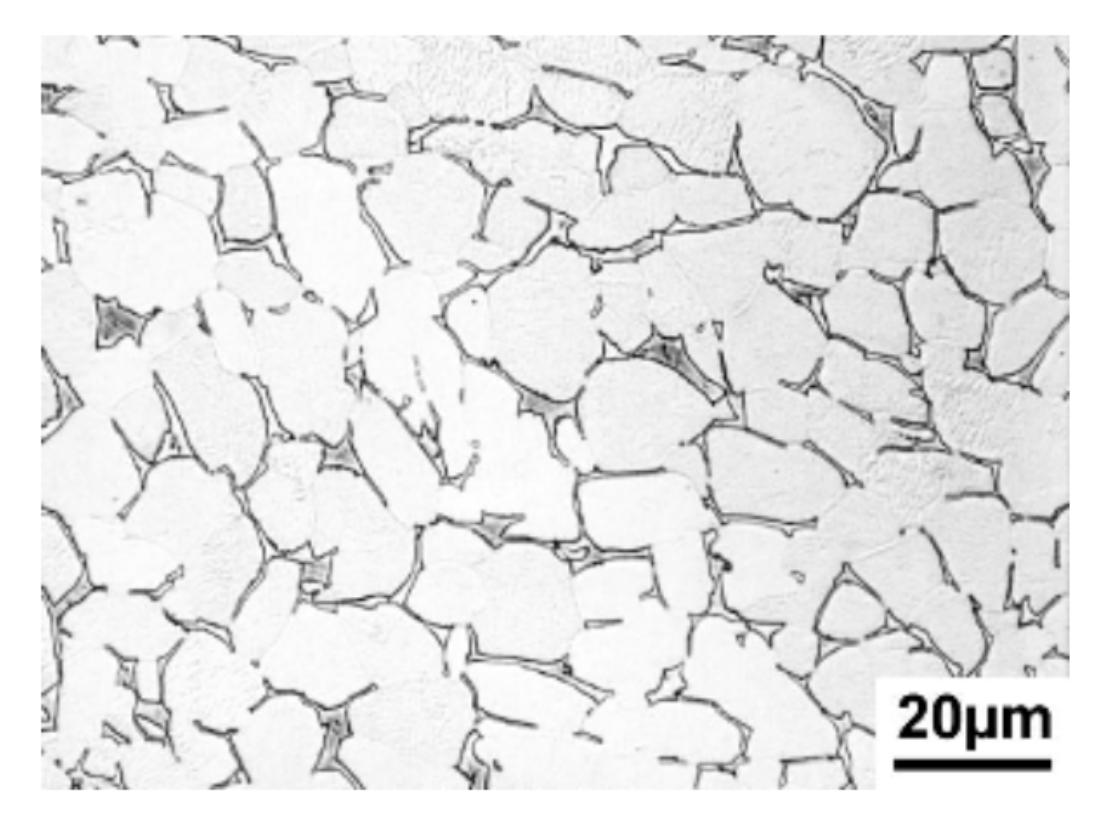
\includegraphics[width=0.7\linewidth]{./Bilder/Abbildung 5.png}
	\caption[Abbildung 5]{globulare Mikrostruktur von Ti-6242, LM \cite{Lutjering.2007}}
	\label{fig:abbildung-5}
\end{figure}

\pagebreak

\begin{figure}[h]
	\centering
	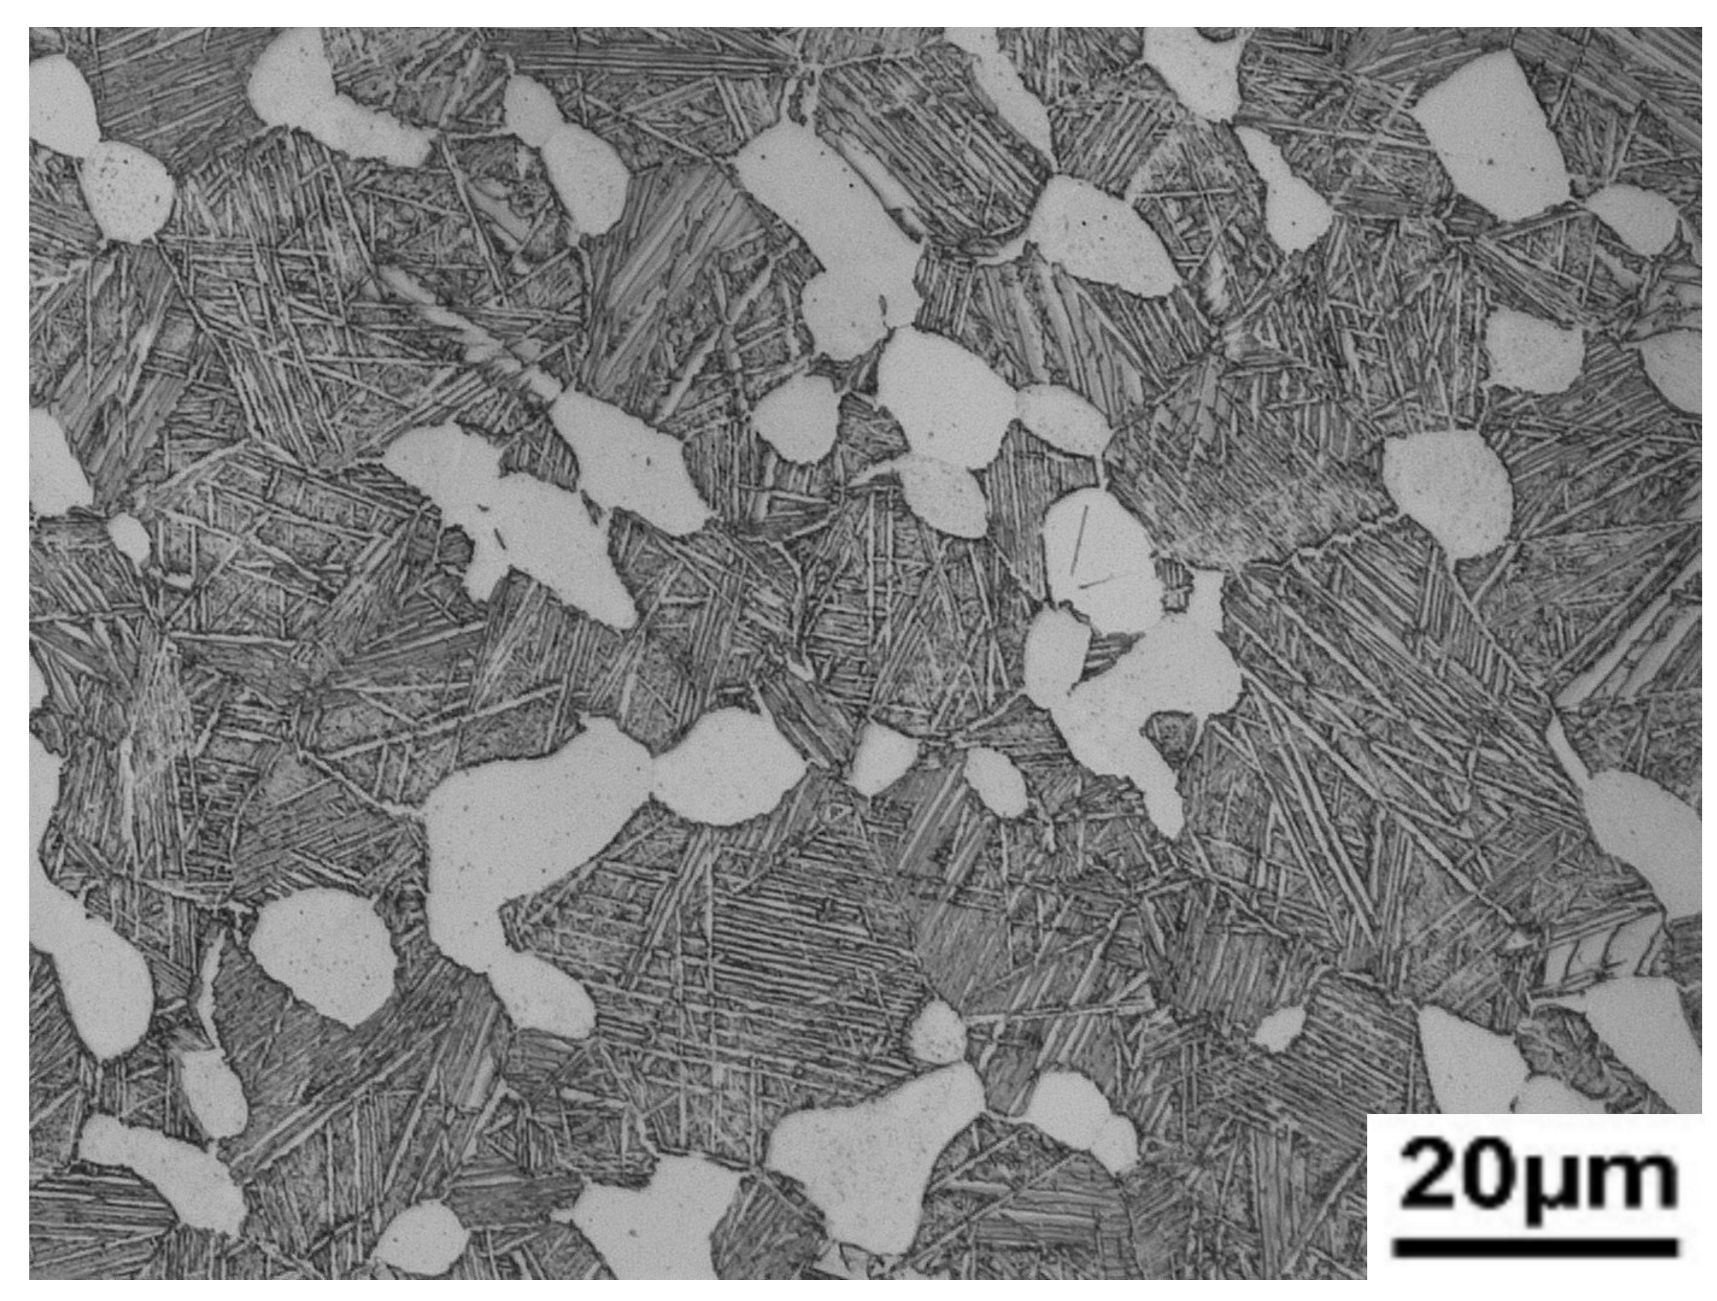
\includegraphics[width=0.6\linewidth]{./Bilder/Abbildung 4.png}
	\caption[Abbildung 4]{bimodale Mikrostruktur Ti-6242}
	\label{fig:abbildung-4}
\end{figure}

\end{itemize} 

Einen Überblick wie diese typischen Mikrostrukturen im quasi-binären Phasendiagramm eingestellt werden können zeigt die Abbildung \ref{fig:gefuge-phasendiagramm}.

\begin{figure}[h]
	\centering
	\includegraphics[width=0.9\linewidth]{./Bilder/Gefüge-Phasendiagramm.png}
	\caption{Quasi-binäres Phasendiagramm Titan mit steigendem Anteil an $\beta$-stabilisierenden
    Legierungselementen und die typischen Mikrostrukturen von $\alpha+\beta$-Legierungen}
	\label{fig:gefuge-phasendiagramm}
\end{figure}

\pagebreak

\subsection{Eigenschaften von Titanlegierungen}

Dieser Abschnitt gibt einen Überblick über die typischen  Eigenschaften der verschiedenen Klassen von Titanlegierungen.

\paragraph{$\alpha$-Legierungen}  
CP-Titanium ist die am weitesten genutzte unter den $\alpha$-Legierungen. Sie besitzen eine annehmbare Zugfestigkeit und gute Duktilität bei Raumtemperatur. Des Weiteren besitzen sie eine geringe Dichte, eine gute Härte, sehr gute Kriechbeständigkeit und Schweißbarkeit. Die Besonderheit dieser Legierungen ist, dass sie bei kryogenen Temperaturen keine Versprödung zeigen \cite{C.Leyens.2005,Lutjering.2007,M.J.Donachie.2010}. 

\paragraph{Near-$\alpha$-Legierungen} 
zeichnen sich durch eine hohe Kriech- und Oxidationsbeständigkeit aus. Ti-6242 ist die am häufigsten kommerziell eingesetzte Legierung für Temperaturen bis zu $450 ^\circ C$. 
Sie wurde als Ergänzung zu der bekannten Ti-64 Legierung entwickelt und erhöhte dadurch das Temperaturlimit. In den meisten near-$\alpha$-Legierungen befindet sich Silizium als Legierungselement, um die Temperaturbeständigkeit zu verbessern \cite{C.Leyens.2005,Lutjering.2007}. 

\paragraph{$\alpha+\beta$-Legierungen} besitzen eine höhere Festigkeit und Härte. Dagegen ist die Duktilität und die Kriechbeständigkeit schlechter als bei near-$\alpha$-Legierungen. Diese Legierungen haben eine hohe Festigkeit bei Raumtemperatur sowie gute Warmumformeigenschaften. Typischerweise besitzen diese Legierungen 10 -- 15 \% $\beta$-Phase bei Raumtemperatur. Ti-64 ist die meistverwendete $\alpha+\beta$-Legierung und besitzt eine gute Kombination aus Festigkeit und Ermüdungseigenschaften bis zu $300 ^\circ C$ \cite{Boyer.2007,M.J.Donachie.2010}. 

Die beschriebenen Eigenschaften der verschiedenen Legierungen sind jedoch abhängig von den zugefügten Legierungselementen sowie dem gewählten Herstellungsprozess.
Die Legierungselemente entscheiden größtenteils über die mechanischen und chemischen Eigenschaften (Korrosion, Oxidation) \cite{C.Leyens.2005,Lutjering.2007,M.J.Donachie.2010}.

Der Herstellungsprozess hat ebenfalls einen erheblichen Einfluss auf die mechanischen Eigenschaften der Legierungen. Durch verschiedene Wärmebehandlungen können dadurch unterschiedliche Mikrostrukturen eingestellt und ihre mikrostrukturellen Eigenschaften verändert werden \cite{C.Leyens.2005,Lutjering.2007,Boyer.2007,M.J.Donachie.2010}.

Wie im vorherigen Kapitel erwähnt, werden drei Basis-Mikrostrukturen unterschieden. Neben $\alpha$- und $\beta$-Phase kann Titan in weiteren Phasen auftreten, wie dem thermisch induzierten Martensit, der als $\alpha'$-Phase bezeichnet wird. Die wichtigsten Eigenschaften der Mikrostrukturen werden durch die Größe der $\alpha$-Lamellenpakete und die Breite der $\alpha$-Lamellen beeinflusst \cite{C.Leyens.2005,Lutjering.2007,Boyer.2007}. Die Größe der $\alpha$-Lamellenpakete, die durch verschiedene Abkühlraten beeinflusst wird, ist der wichtigste mikrostrukturelle Faktor. Es hat sich gezeigt, dass eine Verringerung der Lamellenpaketgröße, zu einer Verringerung der effektiven Gleitlänge führt. Dadurch wird die Dehngrenze erhöht und die Rissanfälligkeit verringert. Größere $\alpha$-Lamellenpakete erhöhen dagegen den Widerstand gegen Ermüdungsrissausbreitung und die Bruchzähigkeit. Die Größe der $\alpha$-Lamellenpakete wird durch die Größe des ursprünglichen $\beta$-Korns limitiert \cite{C.Leyens.2005,Lutjering.2007,M.J.Donachie.2010}.

\subsection{Verwendung von Titan und Titanlegierungen}
Titanlegierungen werden hauptsächlich in der Luft- und Raumfahrt verwendet, da sie eine gute Kombination aus einem niedrigen Gewicht, hoher Festigkeit, Korrosionsbeständigkeit und einer hohen Temperaturstabilität bieten \cite{C.Leyens.2005,R.R.Boyer.1996,M.PetersJ.KumpfertC.WardC.Leyens.2003}. Die Haupteinsatzgebiete in der Luftfahrt für Titanlegierungen sind Strukturteile der Luftfahrzeugzelle, Fahrwerksteile sowie Komponenten von Flugtriebwerken. Etwa 7 -- 36 \% des strukturellen Gewichts des Rumpfes und der Triebwerke bestehen aus Titanlegierungen \cite{Lutjering.2007}. In Triebwerken werden sie für Triebwerksschaufeln eingesetzt. Für die meisten Komponenten wird die Standardlegierung Ti-6Al-4V verwendet. Für Komponenten, die eine höhere Temperaturbeständigkeit erfordern, werden Legierungen wie Ti–6Al–2Sn–4Zr–2Mo und IMI 834 eingesetzt. Die hohen Material- und Herstellungskosten verhindern einen breiten Einsatz von Titanwerkstoffen in der Automobilindustrie. Sie werden aber vereinzelt für Motorkomponenten oder Fahrwerksteile, wie beispielsweise Federn benutzt. Technisch reines Titan (CP-Titanium) findet Anwendung in Bereichen, wo die Anforderungen an mechanische Eigenschaften gering, aber eine hohe Korrosionsbeständigkeit gefordert ist. Beispiele dafür sind Wärmetauscher, Rohrleitungen oder Meerwasserentsalzungsanlagen \cite{A.D.Khawajia.2008}. Des Weiteren finden CP-Titanium und Titanlegierungen Anwendung in der Medizintechnik, aufgrund der Biokompatibilität von Titan sowie einer guten Dauerfestigkeit und Korrosionsbeständigkeit. Sie werden zur Herstellung von Implantaten sowie medizinischen Geräten benutzt \cite{M.GeethaA.K.SinghR.AsokamaniA.K.Gogia.2009}. Ein weiteres Einsatzgebiet sind moderne Schutzwesten, die neben den Aramidfasern auch Titangewebe enthalten, um das Eindringen von Hieb- und Stichwaffen zu verhindern \cite{C.Leyens.2005}.  

\chapter{Experimentelle Methoden}

\section {Metallografische Präparation (VR)}

\subsection*{Trennen}

Die wärmebehandelten Proben werden in der Mitte mit einer Siliziumkarbid-Scheibe unter ständigem Kühlmittelfluss im Querschliff getrennt (Trennmaschine Jean Wirtz CUTO 20). Durchgehende Kühlung  verhindert eine zusätzliche, ungewollte Gefügeveränderung an der Schnittfläche während des Trennvorgangs.


\subsection*{Einbetten}

Die getrennten Proben werden in Warmeinbettpressen (Buehler Simplimet Mounting Press 1000 und 4000) für bessere Handhabung und Stützung der Randzonen eingebettet. Beim Warmeinbetten wird mit Hilfe von Druck und Temperatur die Probe in ein Kunststoffgranulat eingeschlossen. Vorteile des Warmeinbettens sind die hohe Härte und Spaltfreiheit des Einbettmaterials. Dabei wird Epomet als erste Schicht im Bereich der Probenoberfläche benutzt und für die oberflächenfernen Bereiche Bakelit, da Epomet eine bessere Spaltfüllung hat. Das Warmeinbetten erfolgte mit den gerätespezifischen Parametern aus Tab.~\ref{tab:Einbettpressen}. 
Die fertig eingebetteten Proben werden entgratet und auf der Seite der Probenoberfläche mit einer Fase versehen.  


\begin{table}
	\centering
	\begin{tabular} {|c|c|c|}
		\hline
		&Bühler Simplimet 1000 & Bühler Simplimet 4000 \\
		\hline
		Temperatur [$^\circ$ C]&200&180 \\
		\hline
		Druck [bar]&200&200 \\
		\hline
		Haltezeit [min]&5&7 \\
		\hline
		
	\end{tabular}
	
	\caption{Einbettparameter für Bühler Simplimet 1000 und 4000}
	\label{tab:Einbettpressen}
\end{table}

\subsection*{Schleifen/Polieren}

Die Trennfläche der Proben wird in Vorbereitung auf die Ätzung der Oberfläche geschliffen und poliert. Ziel ist eine Oberfläche, die frei von Riefen und Fremdpartikeln ist. Als Schleif-/~Poliergerät wurde ein ATM Saphir 550 benutzt.
Im ersten Schritt werden die Proben mit steigender Körnung im Gegenlauf geschliffen und dabei wassergekühlt (siehe Tab. \ref{tab:Schleifstufen}). Der Probenhalter und Schleifteller haben beide eine Umdrehungszahl von 150 min$^{-1}$, die während des gesamten Schleif- und Polierprozesses gleich bleibt.   

\begin{table}[]
	\centering
	\begin{tabular}{|c|c|c|c|c|c|c|c|c|}
		
		\hline 
		Körnung (FEPA P) & 180 & 240 & 320 & 400 & 600 & 800 & 1200 & 2500 \\ 
		\hline 
		Zeit [min] & 0:30 & 1:00 & 1:30 & 2:00 & 2:30 & 3:00 & 3:30 & 4:00 \\ 
		\hline 
		Anpressdruck [N] & 10&10&10&10&10&10&6&6\\
		\hline
	\end{tabular} 
	\caption{Schleifstufen}
	\label{tab:Schleifstufen}
\end{table}

Zwischen jeder Körnung werden die Proben drei Minuten in einer Seifenlauge ultraschallgereinigt, um größere Schneidkörner und Abrieb nicht zu verschleppen, und die Dauer des Schleifens um 30s verlängert. 

Zum Polieren wird eine Wabenscheibe mit destilliertem Wasser und einer Poliersuspension bestehend aus Oxid-Polier-Suspension (0.05$\mu$m) und Wasserstoffperoxid im Verhältnis 5:1 benetzt. Jede Minute wird Poliersuspension nachgegeben, um eine kontinuierliche Politur zu gewährleisten.

\begin{table}[h]
	\centering
	
	\begin{tabular}{|c|c|c|c|}
		\hline 
		Schritt & Druck [N] & Zeit [min] & Richtung \\ 
		\hline 
		1 & 7 & 5 & Gegenlauf \\ 
		\hline 
		2 & 5 & 2 & Gleichlauf \\ 
		\hline 
	\end{tabular} 
	\caption{Polierstufen}
	\label{tab:Polierstufen}
\end{table}

Die Proben werden nach jedem Schritt (siehe Tab. \ref{tab:Polierstufen}) vier Minuten in einem Ethanolbad ultraschallgereinigt. Nach beiden Polierschritten wird die Wabenscheibe mit Spülmittel gesäubert und die Schritte 1 und 2 wiederholt. Es wird solange poliert bis die Probenoberfläche frei von Riefen und Fremdpartikeln ist. Im letzten Schritt wird die Probenoberfläche nach der Ultrasschallreinigung mit Spülmittel und anschließend mit Ethanol gereinigt und getrocknet. 



\subsection*{Ätzen}

Im letzten Schritt der Probenpräparation werden die Oberflächen der Trennfläche geätzt. Die polierte Oberfläche der Proben reflektiert Licht nahezu gleichmäßig, wodurch das Gefüge der Legierung nicht zu erkennen ist. Das Ätzen erzeugt einen Kontrast zwischen den verschiedenen Mikrostrukturen des Gefüges durch die unterschiedlichen Korrosionsraten der einzelnen Bestandteile \cite{Lutjering.2007}. Stärker korrodierte Gefügebestandteile sind dunkler bei lichtmikroskopischer Betrachtung.
Die Proben werden in einem Ätzmedium nach Kroll (siehe Tab. \ref{tab:Ätz_Kroll}) 7s, martensitische Proben 10s lang geätzt. 

\begin{table}
	\centering
	\begin{tabular}{|c|c|}
		
		\hline 
		Destilliertes Wasser
		& 100ml
		\\ 
		\hline 
		Salpetersäure (HNO$_{3}$)	& 6ml
		\\ 
		\hline 
		Flusssäure (HF) & 3ml
		\\ 
		\hline 
	\end{tabular} 
	\caption{Ätzlösung nach Kroll}
	\label{tab:Ätz_Kroll}
\end{table}

\section{Untersuchung der Mikrostruktur (TJ)}

\subsection*{Lichtmikroskopie}

Nach der Probenpräparation werden die Proben unter dem Lichtmikroskop untersucht. Für die Untersuchung wurde das Zeiss AX10 Lichtmikroskop verwendet. Es werden Bilder mit 200-facher bis 1000-facher Vergrößerung aufgenommen, welche mit ihrem Datennamen und Auflösung beschriftet werden. Anschließend werden verschiedene Stellen untersucht, um die Mikrostrukturen der Proben besser erfassen zu können.

Die einzelnen Phasenanteile können mit Hilfe der verschiedenen Graustufen differenziert und analytisch ausgewertet werden. Dazu können Filter eingesetzt werden, um bestimmte Mikrostrukturen besser hervorzuheben. Es werden \textit{Differential Interference Contrast in circularly polarized lights} (C-DIC) benutzt. Sie sorgen für eine sehr hohe Kontrastdifferenz. Bei mehrphasigen Proben werden sie häufig verwendet, da durch eine Polarisation des Lichtes die Gefüge, insbesondere die Korngrößen- und Phasenanteilbestimmung, optisch besser auswertbar sind.

\subsection*{Rasterelektronenmikroskopie (REM)}

Das Rasterelektronenmikroskop wird benutzt, um eine dreidimensionale Darstellung der Oberfläche zu erzeugen. Das REM Hitachi Tabletop Microscope TM3000 steht mit zwei Freiheitsgraden Verfügung (X-, Y-Richtung). Das Mikroskop ermöglicht höhere Auflösungen gegenüber dem Lichtmikroskop und bietet die Möglichkeit Oberflächen, Materialien sowie die chemische Zusammensetzung zu analysieren. 

Die Proben werden in einer Vakuumkammer untersucht. Im REM werden Elektronen zwischen einer Anode und einer Kathode durch eine angelegte Spannung beschleunigt. Mit Hilfe von magnetischen Linsen werden die ausgestrahlten Elektronen auf die Probenoberfläche fokussiert. 
Die Elektronen, die von der Probenoberfläche zurückkommen, werden detektiert und zu einem Bild verabeitet. 
Um dieses Bild zu erzeugen, werden ausgeschlagene sekundäre Elektronen (SE) detektiert. Diese SE Informationen werden aus der Oberfläche entnommen und in ein Abbild umgewandelt. 
Es lässt sich damit eine dreidimensionale Darstellung der Probenoberfläche erzeugen, je nach Topographie der untersuchten Fläche.

Unter anderen kann das REM mehrere Informationen über die Probe verarbeiten. Eine Veranschaulichung des Massenverhältnisses der Elemente wird mit dem Rückstreuelektronen-Detektor (\textit{Backscatter Electrons}, BSE) bestimmt. Unterschiedliche Phasen erzeugen aufgrund ihrer chemischen Zusammensetzung unterschiedlich starke Kontraste. Die Helligkeit der Bilder wird durch die Anzahl der Elektronen bestimmt.

Die chemische Zusammensetzung der Legierung kann mithilfe der Energiedispersiven Röntgenspektroskopie (EDX) erfasst wird. Aus den inneren Schalen der Atome werden Elektronen ausgestoßen, wodurch Energie freigesetzt wird. Diese Energie wird bei einer EDX-Analyse mit Hilfe eines Siliziumkristalls, der mit flüssigem Stickstoff gekühlt wird, gemessen. Das entstehende Spektrum zeigt dann die Zusammensetzung der Legierung. Es werden an unterschiedlichen Stellen der Probe Flächenanalysen erstellt, um möglichst genaue Daten zu erhalten.

\subsection*{\textit{Field emission} REM}
Für eine bessere Auflösung bei hoher Vergrößerung steht der Smart SEM LEO 1550 zur Verfügung. Die Probenaufnahme der Prozesskammer besitzt 5 Freiheitsgrade (X-, Y-, Z-Richtung, Neigung, Rotation) und mit dem Programm Gemini betrieben. Die Bilder sind entweder mit SE-Detektoren (SE2) erzeugt, oder mit dem Inlens Detektor (hohe Auflösung). Das FE REM hat einen ähnlichen Aufbau und funktioniert wie das zuvor erklärte REM.

Es werden Bilder an verschiedenen Stellen der Probe aufgenommen. Im Mittelbereich und am Rand werden diese mit 2000- bis 20000-facher Vergrößerung untersucht. Polierartefakte können bei der Analyse mit Gefügebestandteilen verwechselt werden. 

\subsection*{$\alpha_{p}$-Volumenanteil Analyse}

Die Bilder vom Lichtmikroskop werden mit Hilfe des Bildbearbeitungsprogramms GIMP analysiert. Zunächst werden die Phasen auf den Bildern durch gezielte Kontrasteinstellung voneinander abgehoben. Im Histogramm können dann die durch die unterschiedlichen Graustufen repräsentierten Gefügebestandteile abgelesen werden. Durch die Analyse von acht verschiedenen Stellen wird ein Mittelwert des $\alpha_{p}$-Volumenanteils mit einer Genauigkeit von 3\% ausgewertet.


\section{Mechanische Prüfverfahren (VR)}

\subsection*{Härteprüfung}

Die Härte der Proben wurde mit einer Vickers-Prüfung nach DIN Norm 50133 ermittelt. Dabei wird die Eindringhärte des Materials gegenüber eines Eindringkörpers in Form einer gleichseitigen Diamantpyramide gemessen. Die Diamantpyramide hat einen Öffnungswinkel von $136^\circ$ zwischen den Seitenflächen und wird mit 10 kg (98,1 N) statischem Druck 15 s lang in die Probe gedrückt. Über die gesamte Probenlänge verteilt werden fünf Eindrücke erzeugt. Ein Abstand von mindestens dreimal der Eindruckdiagonalen $d$ muss dabei vom Rand und zwischen den Eindrücken eingehalten werden.
Die Eindrücke positioniert der Bediener anhand einer lichtmikroskopoischen Aufnahme mit geringer Vergrößerung in der Software. Mit vergrößerten Aufnahmen der ausgewählten Positionen lässt sich der Fokus auf die Bildebene festlegen. Die Prüfmaschine fertigt die Eindrücke automatisch an und fotografiert diese. Die Software ermittelt die Längen der Diagonalen $d_1$ und $d_2$. Dabei kann eine manuelle Überprüfung des von der Software gewählten Messbereichs vorgenommen werden. Die Vickershärte wird durch

$$HV=\frac {2*0,102*F*\sin \left( \frac{136^\circ}{2}\right) } {d^2} \approx 0,1891 \frac{F}{d^2}$$

mit der Eindruckkraft $F$ in Newton und $d=\frac {d_1 + d_2}{2} $ berechnet. Es kann eine Genauigkeit bis auf 3\% erzielt werden.  Die Härte eines Werkstoffs lässt in den meisten Fällen einen direkten Rückschluss auf die Festigkeit zu. Damit kann ohne einen aufwendigeren Zugversuch eine Umwertung der Härte in die Zugfestigkeit anhand empirischer Werte vorgenommen werden. 

\subsection*{Zugversuch}
Zur Bestimmung wichtiger Werkstoffkennwerte wie der Bruchdehnung, Zugfestigkeit, Dehngrenze und des Elastizitätsmoduls werden Zugversuche durchgeführt. Der Zugversuch ist ein genormtes Standardverfahren (DIN EN ISO 6892-1 Teil B), das zu den quasistatischen, zerstörenden Prüfverfahren gehört. Nach DIN 50125-B5x25 in Größe und Form genormte Proben werden dabei mit einer Spannungsgeschwindigkeit von 10 MPas$^{-1}$ bis zum Bruch gedehnt. Gleichzeitig wird die Längenänderung $\Delta l$ und die Kraft $F$ an der Probe gemessen. Mit der Anfangslänge $l_0$ und dem Anfangsquerschnitt $S_0$ lassen sich Nennspannung $\sigma$ und die Dehnung $\epsilon$ berechnen.

$$\sigma=\frac{F}{S_0}$$

$$\epsilon=\frac{\Delta l} {l_0}$$

Die Nennspannung und Dehnung werden in einem Spannungs-Dehnungs-Diagramm (Abb. \ref{fig:spandehn}) gegeneinander aufgetragen. Das Elastizitätsmodul wird von der Messsoftware an der Stelle größter Steigung mit Hilfe einer Tangente berechnet. 

\begin{figure}
	\centering
	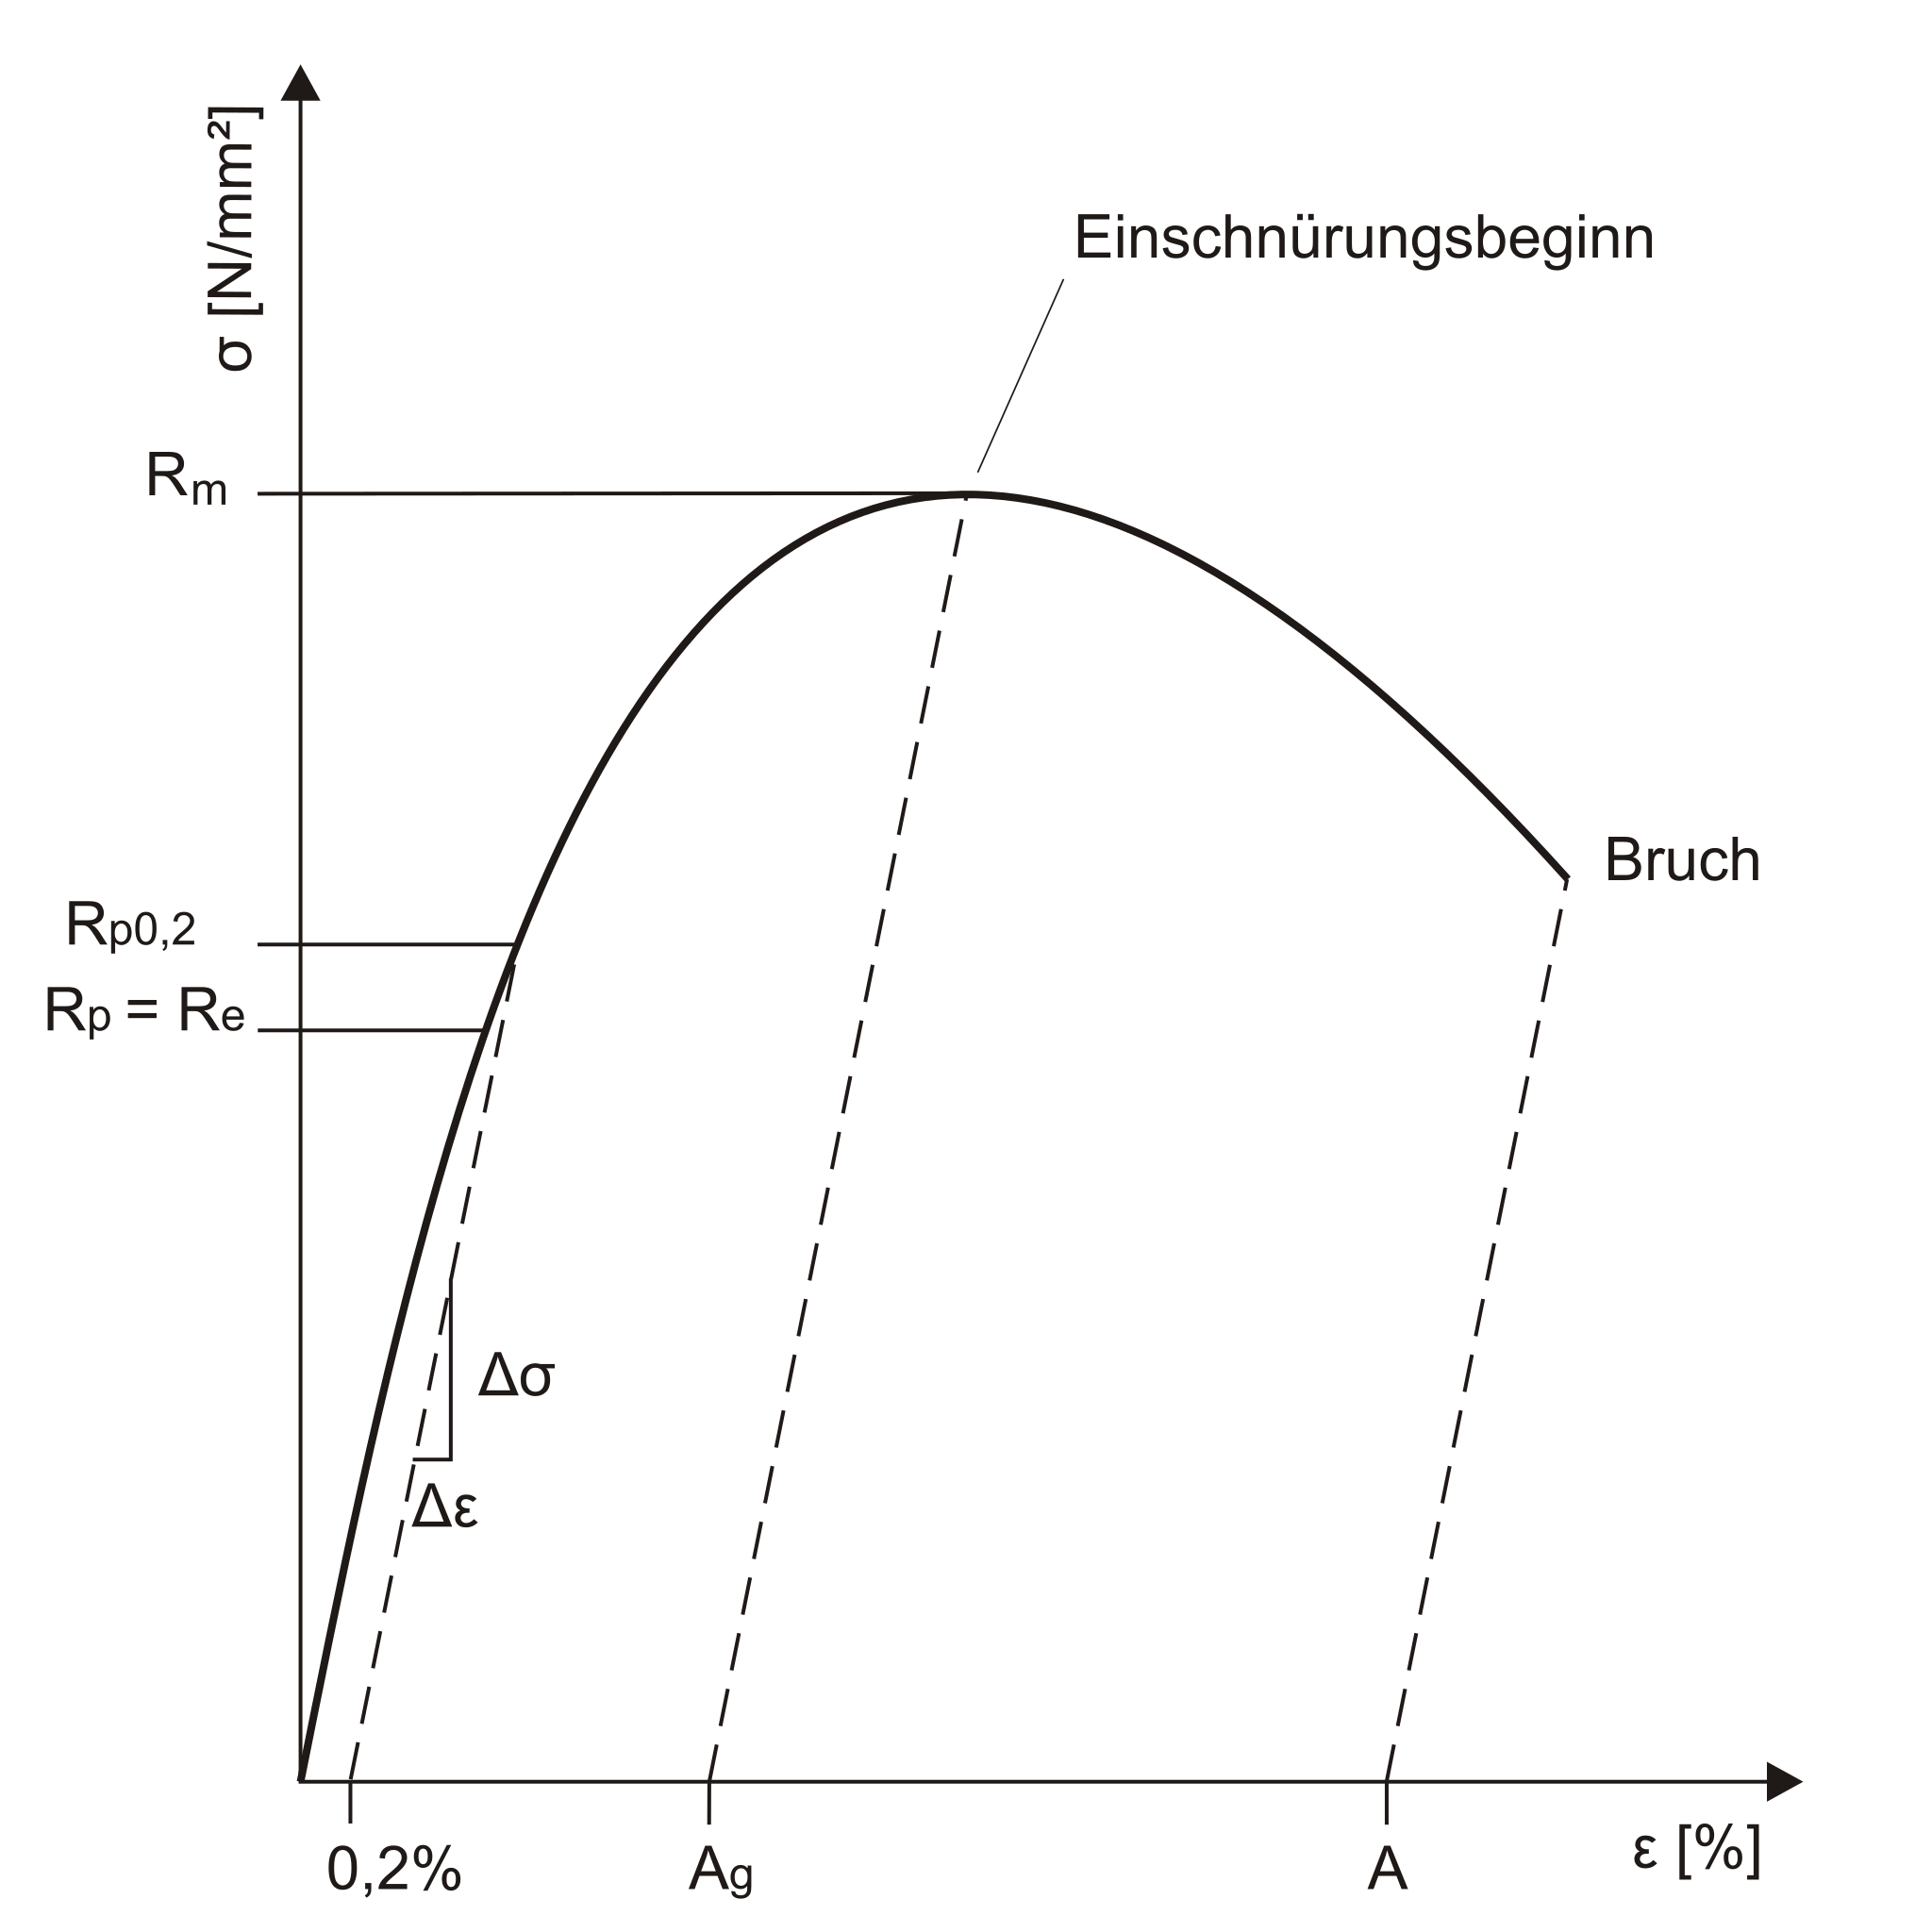
\includegraphics[width=0.6\linewidth]{./Bilder/Spgs-Dehnungs-Kurve_Dehngrenze}
	\caption{Spannungs-Dehnungs-Diagramm}
	\label{fig:spandehn}
\end{figure} 



%\chapter{Durchführung}

\section{$\alpha_p$-Studie (VR)}
Zur Maximierung der Zugfestigkeit der Legierung Ti-6242 wurde zuerst der Einfluss des $\alpha_p$-Phasenanteils auf die Härte untersucht. Laut Lutjering und Williams sollte bei der Legierung IMI 834, eine vergleichbare Legierung zu Ti-6242, eine maximale Zugfestigkeit bei einem $\alpha_p$-Anteil von 10--20\% festgestellt werden \cite{Lutjering.2007}. Um eine größtmögliche Härtesteigerung gegenüber der as-received-Probe (AR) zu erzielen, wurden vier Proben bei unterschiedlichen Temperaturen $1h$ unterhalb der $\beta$-Transus-Temperatur geglüht und anschließend luftgekühlt (AC: air cooled) (\ref{tab:alphap}). Dabei stellt sich ein bimodales Gefüge ein. Die vier Proben wurden inklusive einer AR-Probe metallografisch präpariert und ausgewertet.

\begin{table}
	\centering
	\begin{tabular}{|c|c|c|c|}
	\hline 
	Probenbezeichnung & Temperatur [$^\circ C$] & Zeit [$h$] & Abkühlmethode \\ 
	\hline 
	BM990 & 990 & 1 & AC\\ 
	\hline 
	
	BM975 & 975 & 1 & AC\\ 
	\hline 
	BM960 & 960 & 1 & AC\\ 
	\hline 
	\end{tabular} 
	\caption{Wärmebehandlung der $\alpha_p$-Studie}
	\label{tab:alphap}
\end{table}

\pagebreak

\section{Martensit-Bildung (ZB)}

Um Martensit zu bilden wird Ti-64 nach der ersten Wärmebehandlung laut Abbildung \ref{STDA} für $1 min$  bei $930^\circ C$ geglüht und dann auf Raumtemperatur wassergekühlt. Unter dem Einfluss der Diffusion sollen $\beta$-Lamellen im transformierten $\beta$ wachsen. Die kurze Erwärmungszeit soll dafür sorgen, dass sich die neu gebildeten $\beta$-Gebiete nicht mit $\beta$-Stabilisatoren, in diesem Fall Vanadium, anreichern und dadurch stabilisiert werden. Dieser Prozess läuft im Nanometerbereich ab. Durch das schnelle Abschrecken auf Raumtemperatur wandeln sich die vergrößerten $\beta$-Bereiche diffusionslos und lokal in Martensit um.

\begin{figure}[H]
	\centering
	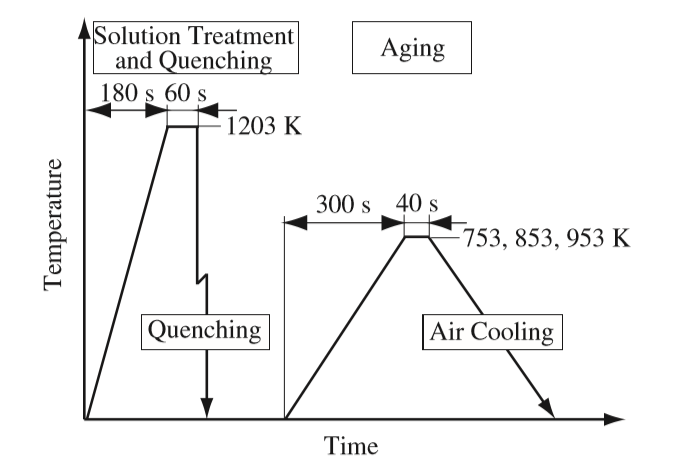
\includegraphics[width=0.9\textwidth]{Bilder/ts-stda}
	\caption{Vorgehensweise nach dem Duplex-Anneal bei STDA für Ti-64 \cite{Morita.2005}}
	\label{STDA}
\end{figure}

Da die $T_{\beta}$ von Ti-64 niedriger ist als die von Ti-6242, liegt auch ihre Gleichgewichtstemperatur unterhalb der von Ti-6242. Außerdem hat Vanadium im Vergleich zu Molybdän eine größere Diffusionsrate in Titan, was die kürzeren Anlasszeiten bei Ti-64 erklärt \cite{Zwicker.2014}. Deswegen wurden in diesem Schritt die Ti-6242-Proben nach dem Duplex-Glühen für 8 und 16 $min$ jeweils bei 930$^\circ$C und $950^\circ C$ wärmebehandelt.

Eine bekannte Wärmebehandlung von $\alpha$+$\beta$-Titanlegierungen ist die  \textit{Solution treatment and quenching}, wobei die Titanlegierung direkt von einer Temperatur $T_{1}$ unterhalb $T_{\beta}$ nach 0,5--1 h abgeschreckt wird. Wie bei der oben beschriebenen Wärmebehandlung stellt sich bei $T_{1}$ ein zweiphasiges Gefüge mit $\alpha_p$ und $\beta$ ein. Die $\beta$-Phase wandelt sich  dann beim Abschrecken martensitisch um und wird $\alpha^\prime$ genannt \cite{Morita.2005}. Zum Vergleich zu der studierten Wärmebehandlung werden AR-Proben bei $983^\circ C$ für 1h erwärmt und wassergekühlt.

\section{Martensit-Zerfall (TJ)}
Um die Härte der Legierung zu steigern, lässt man das Martensit im transformierten $\beta$ partiell zerfallen. Das passiert, indem sich das Martensit in $\alpha$ + $\beta$ umwandelt. Dadurch, dass Martensit Bildung im Nanometer Bereich stattfindet, erfolgt die Bildung mehrere kleine Lamellen. Im Material herrschen extrem kleine Diffusionsvorgänge. Der Martensit ist darin als lokales Gefüge zu finden. Hier für wird für die Wärmebehandlung weniger Zeit benötigt.

Die Probe $983\circ C$ /1h/AC + $950\circ C$ /16min/WQ ist für die nächsten Vorgänge ausgewählt worden. Dazu wurde eine kleine Studie erstellt. Untersucht wurde, ob bei zwei verschiedene Temperaturen einen Anstieg der Härte nachgewiesen werden kann. Dabei wurde sich an den Zeitschriftaufsatz Strengthening of Ti-6Al-4V Alloy by Short-Time Dupelx Heat Treatment von T. Morita, K. Hatsuoka, T. Iizuka und K. Kawasaki orientiert. Die erste Temperatur wurde für die ersten Proben: $580\circ C$ übernommen.Die zweite Temperatur ist um 30K gestiegen ($610\circ C$). Untersucht wurde, ob es einen Unterschied bei einer höheren Temperatur gibt. Für die beiden Schritte sind kurze Zeiten ausgewählt worden. Für die jeweiligen Temperaturen wurden die Proben im Ofen für 8 Minuten bzw. 16 Minuten geglüht. Sie wurden danach im Wasser abgekühlt. 

Der innere Teil der Probe benötigt für die gewünschte Temperatur eine gewisse Zeit. Diese Zeit wird auf 4 Minuten geschätzt. Hierdurch wird erhofft eine Härtesteigerung zu erreichen.

%\chapter {Ergebnisse}

\section{$\alpha_p$-Studie (PH)}

Im Rahmen der Alpha-P Studie wurden zunächst 3 Proben bei verschiedenen Temperaturen unterhalb der Beta-Transus Temperatur (995$^\circ$C für Ti-6242) wärmebehandelt. Ziel war die Einstellung einer bimodalen Mikrostruktur, sowie die Bestimmung des Alpha-Primär-Volumenanteils. Es wurden 3 Temperaturen (990$^\circ$C, 975$^\circ$C und 960$^\circ$C) ausgewählt, bei denen die Proben für eine Stunde im Ofen Wärmebehandelt und anschließend luftabgekühlt wurden. Zusätzlich wurde eine Probe überhalb der Beta-Transus-Temperatur bei 1015$^\circ$C für 30 Minuten geglüht und anschließend in Wasser abgeschreckt, um zum Vergleich der verschiedenen Mikrostrukturen, ein vollmartensitisches Gefüge einzustellen. Die Auswertung dieser Proben unter dem Lichtmikroskop sind in Abbildung 8 aufgeführt. 

\begin{figure}[h]
	\centering
	\includegraphics[width=0.9\linewidth]{"Bilder/Abbildung 8"}
	\caption[Abbildung 8]{Mikrostrukturen der verwendeten Ti-6242 Legierung vor und nach der ersten Wärmebehandlung bei verschiedenen Temperaturen, oben links: Mikrostruktur vor Wärmebehandlung, oben mitte: 960$^\circ$C/1h/AC, oben rechts: 975$^\circ$C/1h/AC, unten links: 983$^\circ$C/1h/AC, unten mitte: 990$^\circ$C/1h/AC, unten rechts: 1015$^\circ$C/30min/WQ vollmartensitisches Gefüge}
	\label{fig:abbildung-8}
\end{figure}

Die Ergebnisse der Bestimmung des Alpha-P Volumenanteils mittels Bildbearbeitungsprogramm sind in Tabelle 4 aufgeführt. Laut Lütjering und Williams liegt der optimale Primär Alpha Volumenanteil zur Steigerung der Zugfestigkeitswerte zwischen 10 und 20 \% [2]. Da die bis dahin erstellten Proben mit ihren Primär Alpha Volumenanteilen außerhalb dieses Bereiches lagen, wurde eine weitere Probe bei 983$^\circ$C für eine Stunde geglüht und anschließend luftgekühlt. Die resultierende Mikrostruktur ist ebenfalls in Abbildung 8 aufgeführt.

\begin{table}[h]
	\centering
	\begin{tabular}{|c|c|}
		\hline 
		& Primär-$\alpha$ in \% \\ 
		\hline 
		AR & 62 \\ 
		\hline 
		960$^\circ$C/1h/AC & 37 \\ 
		\hline 
		975$^\circ$C/1h/AC & 26 \\ 
		\hline 
		983$^\circ$C/1h/AC & 16 \\ 
		\hline 
		990$^\circ$C/1h/AC & 9 \\ 
		\hline 
		1015$^\circ$C/30min/WQ & 0 \\ 
		\hline 
	\end{tabular} 
	\caption{Primär-$\alpha$ Volumenanteile der ersten Wärmebehandlungen mit einer durchnittlichen Abweichung von 3\%}
	\label{Tabelle 4}
\end{table}

Die Auswertung hat ergeben, dass der angestrebte Primär-$\alpha$ Volumenanteil mit der Wärmebehandlung bei 983$^\circ$C für 1 Stunde mit anschließender Luftkühlung erreicht wurde. Die vollmartensitische Probe hat wie erwartet keinen sichtbaren Primär-$\alpha$ Anteil aufgewiesen.


Desweiteren wurde an der ersten Probenreihe eine Härteprüfung durchgeführt. Die Ergebnisse sind zusammen mit der Standardabweichung in Tabelle 5 aufgeführt. 


\begin{table}[h]
	\centering
	\begin{tabular}{|c|c|c|}
		\hline 
		& Härte in HV &  Std.-abw. \\ 
		\hline 
		AR & 331 & 2.45 \\ 
		\hline 
		960$^\circ$C/1h/AC & 345 & 2.83 \\ 
		\hline 
		975$^\circ$C/1h/AC & 344 & 2.80 \\ 
		\hline 
		983$^\circ$C/1h/AC & 344 & 1.84 \\ 
		\hline 
		990$^\circ$C/1h/AC & 350 & 4,74 \\ 
		\hline 
		1015$^\circ$C/30min/WQ & 403 & 3.94 \\ 
		\hline 
	\end{tabular} 
    \caption{Härtewerte der ersten Probenreihe in HV und ihre Standardabweichung}
    \label{Tabelle 5}
\end{table}

Nach der ersten Wärmebehandlung war bei den bimodalen Mikrostrukturen keine wesentliche Härtesteigerung messbar.

\pagebreak

\section{Short Time Duplex Heat Treatment (STDA - short Time Duplex Anneal) (PH)}

Im nächsten Schritt wurde versucht, die STDA Wärmebehandlung von der $\alpha$+$\beta$ Legierung Ti-6Al-4V auf die Near-$\alpha$ Legierung Ti-6AL-2Sn-4Zr-2Mo zu übertragen. Ziel war es zunächst in einem zweiten Prozessschritt Martensit im transformierten Beta zu erzeugen. Dafür wurden die Proben mit bimodalen Mikrostrukturen aus der ersten Wärmebehandlung erneut bei 930$^\circ$C im Ofen für 8 Minuten geglüht und anschließend wassergekühlt. Die Auswertung unter dem Lichtmikroskop ist in Abbildung 9 zusammengefasst.

\begin{figure}[h]
	\centering
	\includegraphics[width=0.9\linewidth]{"Bilder/Abbildung 9"}
	\caption[Abbildung 9]{Mikrostrukturen von Ti-6242 nach dem zweiten Prozessschritt}
	\label{fig:abbildung-9}
\end{figure}

Nach dem zweiten Prozessschritt konnte keine Veränderung der Mikrostrukturen unter dem Lichtmikroskop festgestellt werden. Daher wurden die Proben unter dem Rasterelektronenmikroskop (REM) näher untersucht, um festzustellen, ob sich Martensit im transformierten Beta geformt hat. Die Ergebnisse sind in Abbildungen 10-13 aufgeführt.

\pagebreak

\begin{figure}[!]
	\centering
	\includegraphics[width=0.9\linewidth]{"Bilder/Abbildung 10"}
	\caption[Abbildung 10]{960$^\circ$C/1h/AC + 930$^\circ$C/8min/WQ, REM unter verschiedenen Auflösungen, Randbereich}
	\label{fig:abbildung-10}
\end{figure}

\begin{figure}[!]
	\centering
	\includegraphics[width=0.9\linewidth]{"Bilder/Abbildung 11"}
	\caption[Abbildung 11]{975$^\circ$C/1h/AC + 930$^\circ$C/8min/WQ, REM unter verschiedenen Auflösungen, Randbereich}
	\label{fig:abbildung-11}
\end{figure}

\begin{figure}[!]
	\centering
	\includegraphics[width=0.9\linewidth]{"Bilder/Abbildung 12"}
	\caption[Abbildung 12]{983$^\circ$C/1h/AC + 930$^\circ$C/8min/WQ, REM unter verschiedenen Auflösungen, Randbereich}
	\label{fig:abbildung-12}
\end{figure}

\begin{figure}[!]
	\centering
	\includegraphics[width=0.9\linewidth]{"Bilder/Abbildung 13"}
	\caption[Abbildung 13]{990$^\circ$C/1h/AC + 930$^\circ$C/8min/WQ, REM unter verschiedenen Auflösungen, Randbereich}
	\label{fig:abbildung-13}
\end{figure}

In den Abbildungen 10-13 ist zu erkennen, dass lediglich die Proben der Temperaturenreihe mit 960$^\circ$C und 990$^\circ$C ansatzweise Martensit im Randbereich aufwiesen. Die Proben der Temperaturen mit 975$^\circ$C und 983$^\circ$C zeigten keine Anzeichen von Martensitbildung.

Die Härteprüfung dieser Probenreihe ist in Tabelle 6 zusammengefasst, zeigt jedoch bei keiner Probe eine sichtbare Härtesteigerung.

\begin{table}[h]
	\centering
	\begin{tabular}{|c|c|c|}
		\hline 
		& Härte in HV &  Std.-abw. \\ 
		\hline 
		960$^\circ$C/1h/AC + 930$^\circ$C/8min/WQ & 350 & 2.99 \\ 
		\hline 
		975$^\circ$C/1h/AC + 930$^\circ$C/8min/WQ & 345 & 3.94 \\ 
		\hline 
		983$^\circ$C/1h/AC + 930$^\circ$C/8min/WQ & 349 & 3.19 \\ 
		\hline 
		990$^\circ$C/1h/AC + 930$^\circ$C/8min/WQ & 352 & 4.51 \\ 
		\hline 
    \end{tabular} 
	\caption{Ergebnisse der Härteprüfung der zweiten Probenreihe}
	\label{Tabelle 6}
\end{table}

\pagebreak

Da die Ergebnisse dieser Probenreihe nicht den Erwartungen entsprach und die Martensitbildung zu gering war, wurde dieser zweite Schritt der Wärmebehandlung genauer verfolgt. Ab diesem Punkt wurde im ersten Schritt nur noch mit der Temperatur gearbeitet, die in der Alpha-P Studie als Kandidat für den besten Primär-$\alpha$ Volumenanteil, in Hinblick auf die Zugwerte, ermittelt wurde (983$^\circ$C). 

Um den vorherigen Schritt genauer zu analysieren und optimieren zu können, wurden 3 neue Proben wärmebehandelt. Es wurde daher im zweiten Schritt die Haltezeit der vorherigen Probe verdoppelt. Zusätzlich wurden 2 Proben bei den zwei verschieden Haltezeiten (8 und 16 min) mit einer Temperatur geglüht, die um 20$^\circ$C auf 950$^\circ$C angehoben wurde. Die Auswertung unter dem Lichtmikroskop ist in Abbildung 14 zusammengefasst. 

\begin{figure}[h]
\centering
\includegraphics[width=0.9\linewidth]{"Bilder/Abbildung 14"}
\caption[Abbildung 14]{Mikrostrukturen nach der Anpassung der Temperatur und Haltezeit im zweiten Wärmebehandlungsschritt}
\label{fig:abbildung-14}
\end{figure}

Die Proben, die im zweiten Schritt bei 930$^\circ$C geglüht wurden, weisen in ihrer Mikrostruktur keine offensichtlichen Unterschiede zur vorherigen Probenreihe auf. Die Proben, die im zweiten Schritt bei 950$^\circ$C geglüht wurden weisen eine Veränderung in der transformierten $\beta$-Phase auf. So scheint der $\beta$-Phasenanteil im transformierten $\beta$ zwischen den $\alpha$-Lamellen gewachsen zu sein. Eine Gegenüberstellung unter dem Lichtmikroskop ist in Abbildung 15 zu sehen.

\begin{figure}[h]
\centering
\includegraphics[width=0.9\linewidth]{"Bilder/Abbildung 15"}
\caption[Abbildung 15]{Veränderung der transformierten $\beta$-Phase in zweiten Wärmebehandlungsschritt bei 950$^\circ$C und 930$^\circ$C}
\label{fig:abbildung-15}
\end{figure}

Die Härteprüfung der zweiten Probenreihe mit angepassten Temperaturen und Haltezeiten ergab ebenfalls einen Unterschied zur vorherigen Probenreihe. Die Ergebnisse sind in Tabelle 7 aufgeführt.

\begin{table}[h]
\centering
\begin{tabular}{|c|c|c|}
\hline 
& Härte in HV &  Std.-abw. \\ 
\hline 
983$^\circ$C/1h/AC + 930$^\circ$C/8min/WQ & 349 & 3.19 \\ 
\hline 
983$^\circ$C/1h/AC + 930$^\circ$C/16min/WQ & 358 & 7.23 \\ 
\hline 
983$^\circ$C/1h/AC + 950$^\circ$C/8min/WQ & 377 & 3.44 \\ 
\hline 
983$^\circ$C/1h/AC + 950$^\circ$C/16min/WQ & 376 & 3.79 \\ 
\hline 
\end{tabular} 
\caption{Ergebnisse der Härteprüfung mit angepassten Temperaturen und Haltezeiten}
\label{Tabelle 7}
\end{table}

Die Härtewerte der Proben, die bei 950$^\circ$C geglüht wurden, weisen eine sichtbare Härtesteigerung gegenüber den Proben, die bei 930$^\circ$C geglüht wurden, auf. Die Härtesteigerung der Probe, die bei 930$^\circ$C und 16 min geglüht wurde, gegenüber der Probe mit gleicher Temperatur und halber Haltezeit, kann mit der größeren Standardabweichung erklärt werden. So zeigt sich, dass in dieser Probenreihe, die Haltezeit keinen sichtbaren Einfluss hatte.

Die nähere Analyse der Mikrostruktur dieser Probenreihe unter dem Rasterelektronenmikroskop ist in den Abbildungen 16 - 18 aufgeführt.

\begin{figure}[!]
	\centering
	\includegraphics[width=0.9\linewidth]{"Bilder/Abbildung 16"}
	\caption[Abbildung 16]{983$^\circ$C/1h/AC + 930$^\circ$C/16min/WQ, REM unter verschiedenen Auflösungen, Randbereich}
	\label{fig:abbildung-16}
\end{figure}

\begin{figure}[!]
	\centering
	\includegraphics[width=0.9\linewidth]{"Bilder/Abbildung 17"}
	\caption[Abbildung 17]{983$^\circ$C/1h/AC + 950$^\circ$C/8min/WQ, REM unter verschiedenen Auflösungen}
	\label{fig:abbildung-17}
\end{figure}

\begin{figure}[!]
	\centering
	\includegraphics[width=0.9\linewidth]{"Bilder/Abbildung 18"}
	\caption[Abbildung 18]{983$^\circ$C/1h/AC + 950$^\circ$C/16min/WQ, REM unter verschiedenen Auflösungen}
	\label{fig:abbildung-18}
\end{figure}

\pagebreak

Die Analyse hat gezeigt, dass auch bei der Probe, die bei 930$^\circ$C für 16 Minuten geglüht wurde, ebenfalls nur im Randbereich an vereinzelten Stellen in der $\beta$-Phase, leichte martensitische Strukturen erkennbar waren.
Bei den Proben, die bei einer Temperatur von 950$^\circ$C geglüht wurden, sind über der ganzen Probenfläche ausgeprägte martensitische Strukturen ersichtlich. In den Proben mit tieferer Temperatur haben sich lediglich vereinzelt martensitische Strukturen in Bereichen großflächiger $\beta$-Phase im Randbereich gebildet. Bei den Proben, die bei höherer Temperatur geglüht wurden, haben sich auch in den dünneren Flächen der $\beta$-Phase, die zwischen den $\alpha$-Lamellen liegen, ausgeprägte Martensitstrukturen gebildet.

Im dem dritten Schritt war der Zerfall des Martensites, das vorher gebildet wurde, geplant. Dazu wurde die Probe aus Abbildung 18, die die ausgeprägtesten Martensitstrukturen aufwies, für die weiteren Schritte ausgewählt. 
Dafür wurden vier Proben für den dritten Wärmebehandlungsschritt festgelegt. Zwei Proben wurden bei 580$^\circ$C und unterschiedlichen Haltezeiten (8 und 16 min) wärmebehandelt. Die zwei verbliebenen wurden den gleichen Haltezeiten ausgesetzt, nur bei höher Temperatur (610$^\circ$C).

Die Analyse unter dem Lichtmikroskop ergab keine sichtbare Veränderung der Mikrostruktur zur vorherigen Probenreihe.

Die Härteprüfung dagegen zeigte eine sichtbare Härtesteigerung. Die Ergebnisse sind in Tabelle 8 zusammengefasst.

\begin{table}[h]
	\centering
	\begin{tabular}{|c|c|c|}
		\hline 
		& Härte in HV &  Std.-abw. \\ 
		\hline 
		983$^\circ$C/1h/AC + 930$^\circ$C/8min/WQ + 580$^\circ$C/8min/AC & 393 & 2.02 \\ 
		\hline 
		983$^\circ$C/1h/AC + 930$^\circ$C/16min/WQ + 580$^\circ$C/16min/AC & 392 & 4.15 \\ 
		\hline 
		983$^\circ$C/1h/AC + 950$^\circ$C/8min/WQ + 610$^\circ$C/8min/AC & 399 & 2.32 \\ 
		\hline 
		983$^\circ$C/1h/AC + 950$^\circ$C/16min/WQ + 610$^\circ$C/16min/AC & 392 & 2.57 \\ 
		\hline 
	\end{tabular} 
	\caption{Ergebnisse der Härteprüfung mit angepassten Temperaturen und Haltezeiten}
	\label{Tabelle 8}
\end{table}

\pagebraek

\section{$\alpha_p - $\alpha'$ Wärmebehandlung (PH)}

Zum Vergleich wurde parallel eine $\alpha_p$ - $\alpha'$ Wärmebehandlung durchgeführt. Im Gegensatz zur der im Abschnitt 5.2. durchgeführten Wärmebehandlung, besitzt diese nur zwei Behandlungsschritte.
Dazu wurde wieder die aus der $\alpha$-P Studie hervorgegangene Temperatur von 983$^\circ$C ausgewählt, eine Probe für 1 Stunde geglüht und anschließend wassergekühlt. Die dadurch entstandene Mikrostruktur wurde unter dem Lichtmikroskop ausgewertet und ist in Abbildung 19 aufgeführt.

\pagebreak

\begin{figure}[h]
	\centering
	\includegraphics[width=0.9\linewidth]{"Bilder/Abbildung 19"}
	\caption[Abbildung 19]{$\alpha_p - $\alpha'$ Gefüge unter dem Lichtmikroskop bei verschiedenen Auflösungen}
	\label{fig:abbildung-19}
\end{figure}

Der Unterschied in diesem ersten Schritt der Wärmebehandlung zu der Behandlung aus Abschnitt 5.2., liegt in der Wasserabkühlung. Das dadurch entstandene Gefüge besteht aus Primär-$\alpha$ und vollmartensitischer $\beta$-Phase.

Die anschließende Härteprüfung ergab eine mittlere Vickershärte von 405 HV bei einer Standardabweichung von 4.84 \%.

Im zweiten Schritt dieser Vergleichsbehandlung wurde wieder ein Martensitzerfall durchgeführt. Dazu wurden zwei Proben erneut bei 610$^\circ$C wärmebhandelt. Es wurden zwei Haltezeiten bei 16 und 30 Minuten ausgewählt, mit anschließender Luftabkühlung. 

Die Ergebnisse der Härteprüfung nach diesem zweiten Schritt sind in Tabelle 9 aufgeführt.

\begin{table}[h]
	\centering
	\begin{tabular}{|c|c|c|}
		\hline 
		& Härte in HV &  Std.-abw. \\ 
		\hline 
		983$^\circ$C/1h/WQ + 610$^\circ$C/16min/AC & 405 & 6.22 \\ 
		\hline 
		983$^\circ$C/1h/WQ + 610$^\circ$C/30min/AC & 400 & 2.81 \\ 
		\hline 
	\end{tabular} 
	\caption{Ergebnisse der Härteprüfung nach der zweiten Wärmebehandlung, $\alpha_p - $\alpha'$ Gefüge}
	\label{Tabelle 9}
\end{table}



\pagebreak

\section{Zugversuche (PH)}

%\chapter{Diskussion der Ergebnisse}

\section{Martensitbildung}


Im Gegensatz zu der zweiten Probenreihe, war  bei den ersten Proben, die bei 930°C für 8   oder 16 min WQ ..., wenig bis gar kein Martensit zu erkennen. Die Härte ist auch nur leicht gestiegen. Diese kleine Härteverbesserung zeigt aber trotzdem, dass  die Gefügestruktur  beeinflusst wurde. D.h es konnte sich bei 930°C das $\beta$ nicht schnell genug wachsen wie bei Ti64 oder neue $\beta$-Gebiete sind bereits in der kurzen Anlass-zeit  durch Diffusion von Mo stabilisiert worden. 
Das hat dazu geführt, dass sich, wenn überhaupt, nur in bestimmten Nano-Gebieten martensitische Strukturen gebildet haben. Außerdem ist diese Umwandlung nur bei  990/8/WQ-Probe und 960/8/WQ-Probe relativ besser zu sehen. Da die Randbereiche bei der Erwärmung zuerst durchwärmt werden, sind martensitische Strukturen auch am Rand besser erkennbar.
990-Proben haben durch die höhere Rekristallisationstemperatur den höchsten $\beta$-Anteil. Das erklärt, warum sich im Gegensatz zu 983- und 975-Proben zu Martensitbildung gekommen ist.
Bei den 960-Proben konnte sich aber trotzdem, auch wenn nur  lokal, Martensit bilden. Das ist möglicherweise darauf zurückzuführen, dass die Rekristallisationstemperatur  so niedrig war, dass sich Mo nicht vernünftig  in der $\beta$-Phase diffundieren konnte. Dadurch wurden nur beschränkte $\beta$-Gebiete stabilisiert.

Auch bei der Erwärmung für 16 min waren keine signifikante Änderung abzulesen. Das erklärt dass die Dauer des Anlassens bei 930°C nur einen geringen bis keinen Einfluss auf die Martensitbildung hat. 
Bei den anderen Proben hingegen ist die Härte von 344 HV auf 376 HV gestiegen. 
Das zeigt, dass 930°C zu niedrig  für die Diffusionskinetik von $\beta$ war. Das liegt wahrscheinlich daran, dass die Gleichgewichtstemperatur von Ti6242 höher ist als die von Ti64. Die Kinetische Energie von 930 reicht nicht aus um martensit zu bilden bei ti6242.

\paragraph{$\alpha$ + $\alpha^\prime$}

Bei 983°C  liegt die Legierung in dem  Zwei-Phasengebiet mit ca. 84\% $\beta$. Bei der Wasserabschreckung über $M_s$ wandelt sich die ganze $\beta$-Phase martensitisch um. Das hat dann zu einem Signifikanten Härteanstieg geführt. Duktilität ?


\section{Martensitzerfall}
\chapter{$\alpha_p$-Studie}

\section*{As-received-Proben (VR)}

Die Proben sind zylindrische Stangenabschnitte mit einem Durchmesser von 19 mm und einer Höhe von 8 mm. Der Zustand der Proben ist rekristallisationsgeglüht. Eine metallografische Untersuchung des Gefüges zeigt eine globulare Mikrostruktur mit einem $\alpha_p$-Volumenanteil von 62\%. 


\section{Durchführung (VR)}

Zur Maximierung der Zugfestigkeit der Legierung Ti-6242 wurde zuerst der Einfluss des $\alpha_p$-Phasenanteils auf die Härte untersucht. Laut Lütjering \cite{Lutjering.2007} konnte bei der Legierung IMI 834 eine maximale Zugfestigkeit bei einem $\alpha_p$-Anteil von 10--20\% festgestellt werden. \\
Um eine größtmögliche Härtesteigerung gegenüber der as-received-Probe (AR) zu erzielen, wurden vier Proben bei unterschiedlichen Temperaturen 1h unterhalb der $\beta$-Transus-Temperatur geglüht und anschließend luftgekühlt (AC: air cooled) (Tab. \ref{tab:alphap}). Zu erwarten sind abnehmende $\alpha_p$-Volumenanteile mit steigender Temperatur. Zusätzlich wurde eine Probe bei 1015$^\circ$C 30min lang geglüht und wassergekühlt, um ein vollmartensitisches Gefüge einzustellen. Die fünf Proben wurden inklusive einer AR-Probe metallografisch präpariert und ausgewertet.



\begin{table}[h]
	\centering
	\begin{tabular}{|c|c|c|c|}
		\hline 
		Probenbezeichnung & Temperatur [$^\circ$C] & Zeit [h] & Abkühlmethode \\ 
		\hline 
		BM990 & 990 & 1 & AC\\ 
		\hline 
		BM983 & 983 & 1 & AC\\
		\hline
		BM975 & 975 & 1 & AC\\ 
		\hline
		BM960 & 960 & 1 & AC\\ 
		\hline 
		M1015 & 1015 & 0.5 & WQ\\ 
		\hline
	\end{tabular} 
	\caption{Wärmebehandlungen der $\alpha_p$-Studie}
	\label{tab:alphap}
\end{table}



\section{Ergebnisse (PH)}

Im Rahmen der $\alpha_p$-Studie wurden zunächst vier Proben bei verschiedenen Temperaturen unterhalb der $\beta$-Transus-Temperatur (995$^\circ$C für Ti-6242) wärmebehandelt. Ziel war die Einstellung einer bi-modalen Mikrostruktur, sowie die Bestimmung des $\alpha_p$-Volumenanteils. Die Auswertung dieser Proben unter dem Lichtmikroskop ist in Abbildung \ref{fig:abbildung-8} aufgeführt. 

\begin{figure}[h]
	\centering
	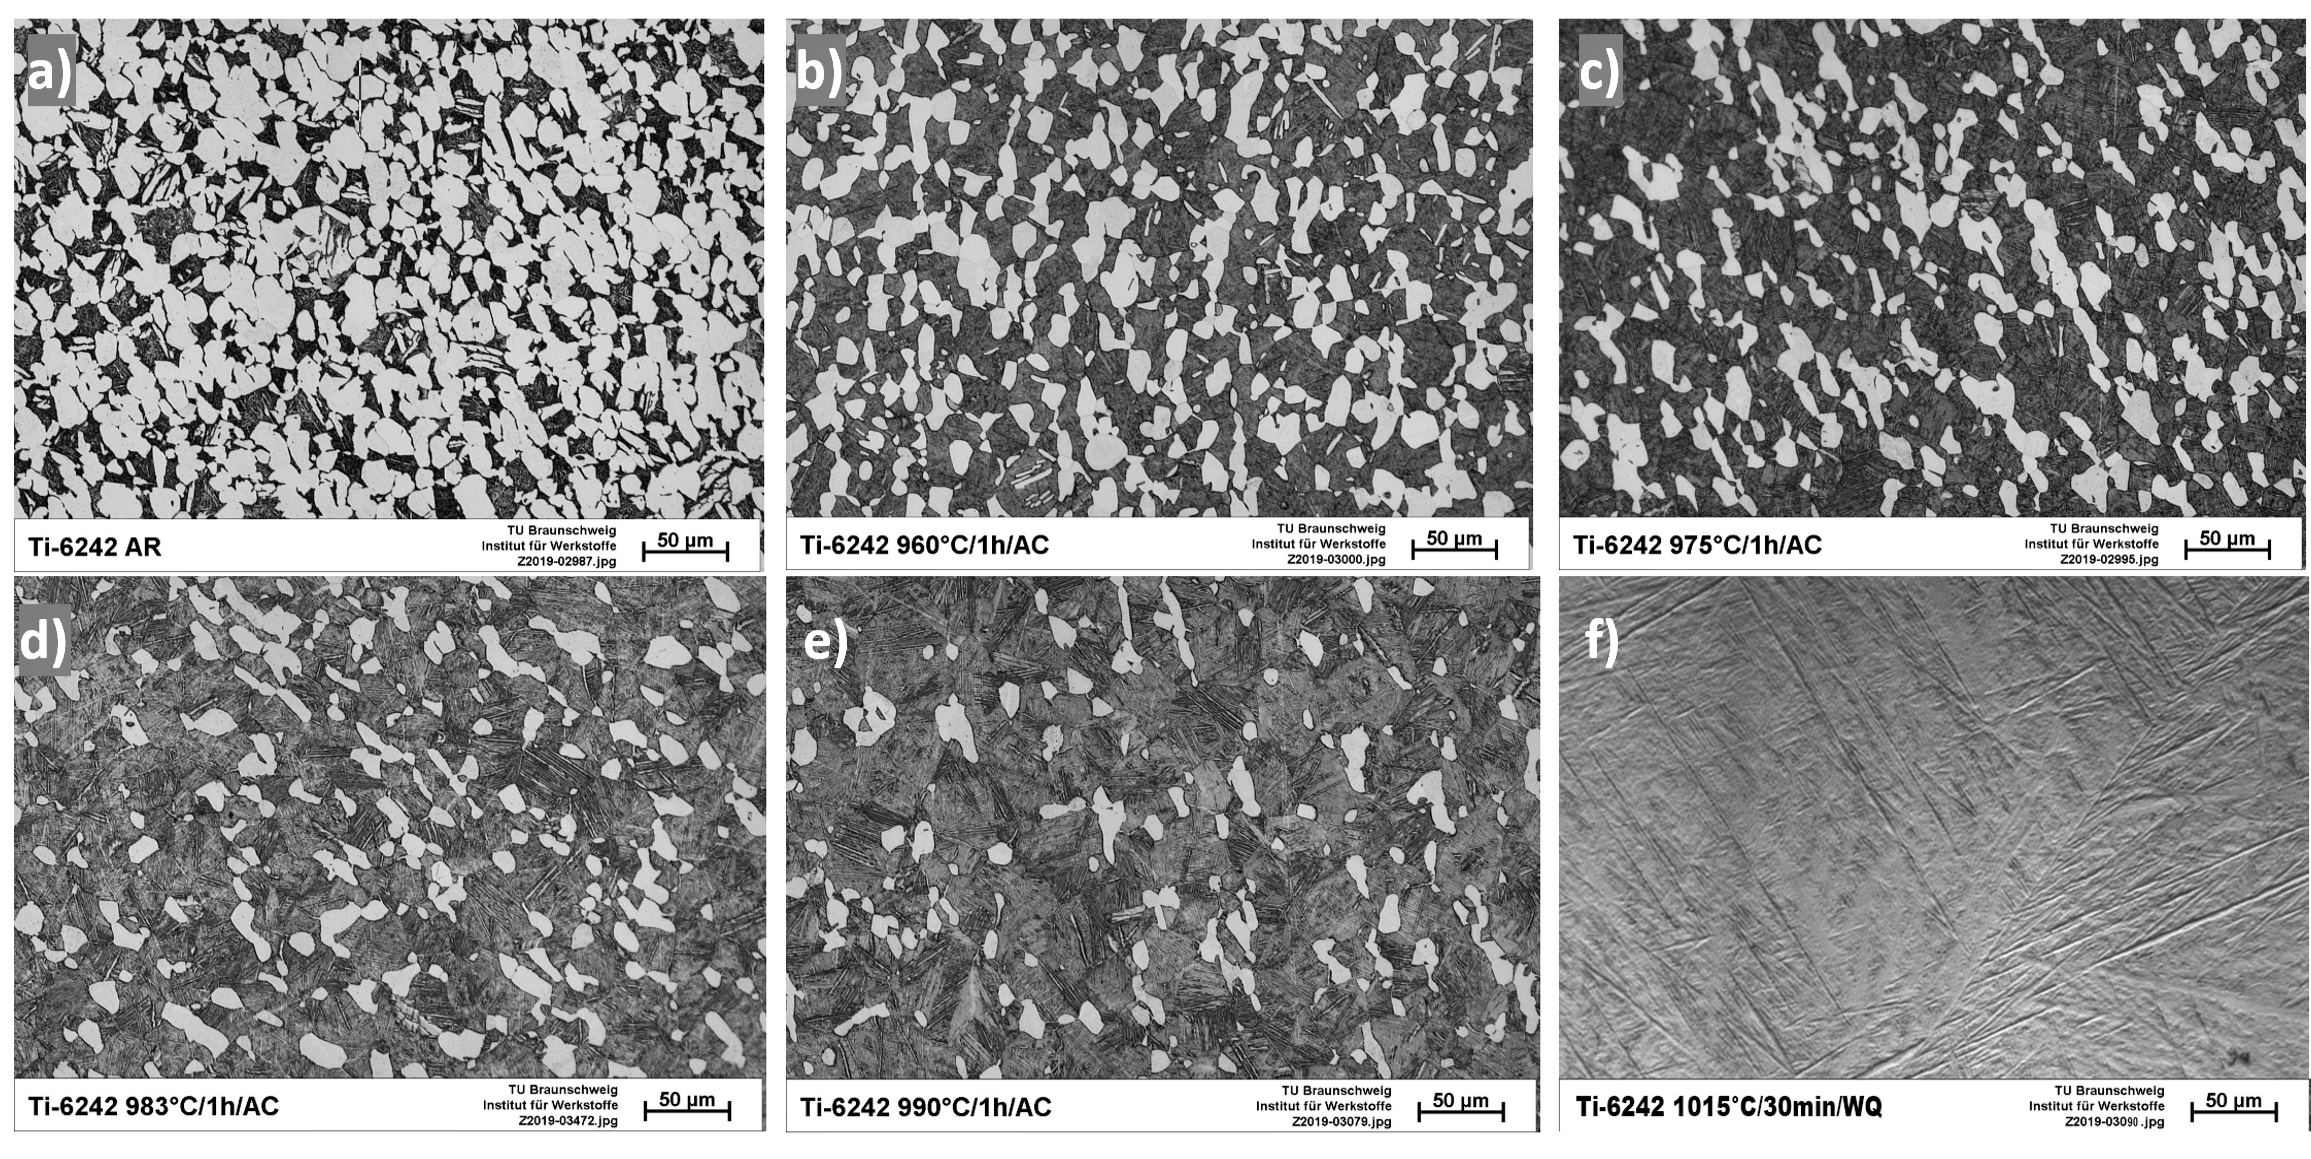
\includegraphics[width=1.0\linewidth]{./Bilder/Abbildung 8.png}
	\caption[Abbildung 8]{Mikrostrukturen der verwendeten Ti-6242 Legierung vor und nach der ersten Wärmebehandlung bei verschiedenen Temperaturen, a) Mikrostruktur vor Wärmebehandlung (AR), b) 960$^\circ$C/1h/AC, c) 975$^\circ$C/1h/AC, d) 983$^\circ$C/1h/AC, e) 990$^\circ$C/1h/AC, f) 1015$^\circ$C/30min/WQ vollmartensitisches Gefüge}
	\label{fig:abbildung-8}
\end{figure}

Ein Überblick über die in der bi-modalen Mikrostruktur auftretenden Gefügebestandteile zeigt die Abbildung \ref{fig:abbildung-20}.

\begin{figure}[h]
	\centering
	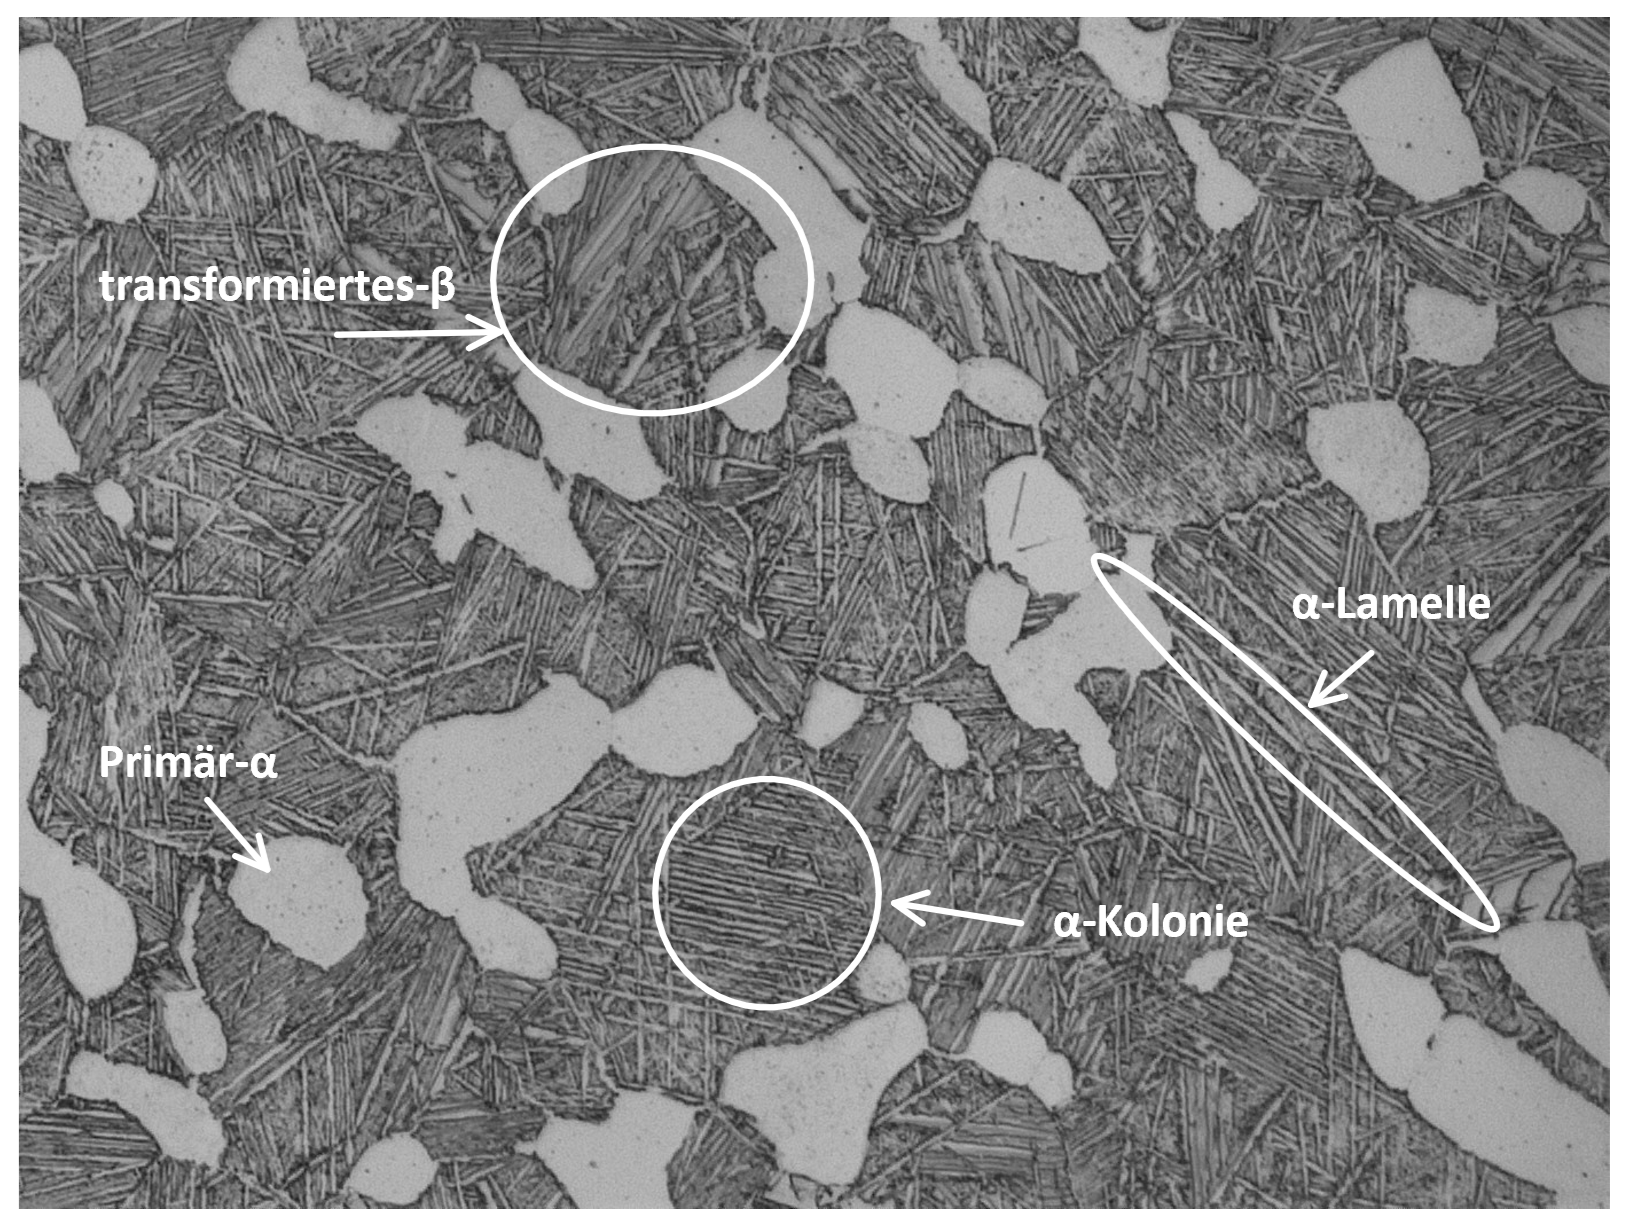
\includegraphics[width=0.6\linewidth]{./Bilder/Abbildung 20.png}
	\caption[Abbildung 20]{Gefügebestandteile in bi-modaler Mikrostruktur}
	\label{fig:abbildung-20}
\end{figure}

Die Ergebnisse der Bestimmung des $\alpha_p$-Volumenanteils mittels Bildbearbeitungsprogramm sind in Tabelle \ref{Tabelle 4} aufgeführt. Laut Lütjering und Williams liegt der optimale $\alpha_p$-Volumenanteil zur Steigerung der Zugfestigkeitswerte zwischen 10 und 20 \% \cite{Lutjering.2007}.

\begin{table}[h]
	\centering
	\begin{tabular}{|c|c|}
		\hline 
		Probe & Primär-$\alpha$ in \% \\ 
		\hline 
		AR & 62 \\ 
		\hline 
		960$^\circ$C/1h/AC & 37 \\ 
		\hline 
		975$^\circ$C/1h/AC & 26 \\ 
		\hline 
		983$^\circ$C/1h/AC & 16 \\ 
		\hline 
		990$^\circ$C/1h/AC & 9 \\ 
		\hline 
		1015$^\circ$C/30min/WQ & 0 \\ 
		\hline 
	\end{tabular} 
	\caption{$\alpha_p$-Volumenanteile der ersten Wärmebehandlungen mit einer Genauigkeit von 3\%}
	\label{Tabelle 4}
\end{table}

Die Auswertung hat ergeben, dass der angestrebte $\alpha_p$-Volumenanteil mit der Wärmebehandlung bei 983$^\circ$C für 1 h mit anschließender Luftkühlung erreicht wurde. Die vollmartensitische Probe hat wie erwartet keinen sichtbaren $\alpha_p$-Anteil aufgewiesen.


Des Weiteren wurde an der ersten Probenreihe eine Härteprüfung durchgeführt. Die Ergebnisse sind in Tabelle \ref{Tabelle 5} aufgeführt. 

\begin{table}[h]
	\centering
	\begin{tabular}{|c|c|}
		\hline 
		Probe & Härte in HV \\ 
		\hline 
		AR & 331 \\ 
		\hline 
		960$^\circ$C/1h/AC & 345 \\ 
		\hline 
		975$^\circ$C/1h/AC & 344 \\ 
		\hline 
		983$^\circ$C/1h/AC & 344 \\ 
		\hline 
		990$^\circ$C/1h/AC & 350 \\ 
		\hline 
		1015$^\circ$C/30min/WQ & 403 \\ 
		\hline 
	\end{tabular} 
	\caption{Härtewerte der ersten Probenreihe in HV}
	\label{Tabelle 5}
\end{table}

Nach der ersten Wärmebehandlung war bei den Proben mit bi-modaler Mikrostruktur eine geringe Härtesteigerung gegenüber der AR-Probe festzustellen. 
Die Probe mit vollmartensitischem Gefüge hat dagegen eine signifikante Härtesteigerung gezeigt. Dies kann durch die feinere Struktur des Martensits und dadurch erhöhte Grenzflächendichte begründet werden. Sie wurde aber im Rahmen der gewählten Strategien nicht weiter verfolgt, da bi-modale Gefüge im Hinblick auf die zu erreichende Bruchdehnung (mind. 10\%) eine bessere Basis darstellen.


\section{Diskussion der Ergebnisse (VR)}

Es zeigt sich, dass mit steigender Glühtemperatur der $\alpha_p$-Anteil geringer wird. Eine Temperatur näher an T$_{\beta}$ bedeutet einen größeren $\beta$-Phasenanteil im Gleichgewichtszustand, die bei Abkühlung teilweise in lamellares $\alpha$ transformiert. Die Glühzeit hat dabei keinen Einfluss die Mikrostruktur. Sie muss nur lang genug sein für die Bildung von isolierten, globularen $\alpha_p$-Körnern \cite{G.LutjeringJ.C.WilliamsA.Gysler.}. 
Die Werte zeigen eine Erhöhung der Härte gegenüber den AR-Proben, aber keine signifikanten Unterschiede untereinander. Die Lamellenpakete sind durch ihre feine Mikrostruktur härter gegenüber dem gröberen $\alpha_p$-Körnern, sodass ein Härteanstieg mit sinkendem $\alpha_p$-Volumenanteil zu erwarten wäre. Da die $\alpha_p$-Körner eine Wachstumsbehinderung für die transformierte $\beta$-Phase darstellen und somit die Lamellenpaketbreite begrenzen, bedeutet ein geringerer Anteil eine größere Weglänge zwischen einzelnen Körnern. Somit kommt es zu weniger Grenzflächen zwischen dem $\alpha_p$ und transformiertem $\beta$ und einer Festigkeitsabnahme. Diese zwei gegenläufigen Effekte erklären die annähernd gleichen Härtewerte für alle vier Temperaturen der Wärmebehandlung. 
\chapter{Martensitbildung}

\section{Durchführung}
\section{Ergebnisse}
\section{Diskussion der Ergebnisse}
\chapter{Martensitzerfall}

\section{Durchführung}
\section{Ergebnisse}
\section{Diskussion der Ergebnisse}
\chapter{Strategie 2}

\section{Durchführung (ZB)}

Eine bekannte Wärmebehandlung von $\alpha$+$\beta$-Titanlegierungen ist die  \textit{Solution treatment and quenching + Aging}(Abbildung \ref{fig:SQ}). Im Gegensatz zu  Strategie 1 wird hier ein Duplex-Glühen zum Einstellen eines bi-modalen Gefüges nicht gebraucht. Werkstücke werden im ersten Schritt bei einer Temperatur unterhalb $T_{\beta}$ für 1--2 h geglüht und danach wassergekühlt. Es wurde auch bei dieser Strategie die aus der $\alpha_p$-Studie ermittelte Temperatur von 983$^\circ$C für 60 min gewählt, damit sich vergleichbare $\alpha_p$-Volumenanteile einstellen. Durch das Abschrecken wandelt sich die $\beta$-Phase martensitisch um.

Um das Gefüge noch weiter zu verfeinern, wird der zweite Wärmebehandlungsschritt, das Anlassen, durchgeführt. Hier sollen die Proben nochmal erwärmt und dann luftgekühlt werden. Bei der erhöhten Temperatur soll sich der Martensit in $\beta$- und $\alpha$-Körner umwandeln.
Um beide Strategien noch besser vergleichen zu können werden in diesem Schritt die Proben bei  610$^\circ$C für 16 und 30 min angelassen und anschließend luftgekühlt.

\begin{figure}[h]
	\centering
	{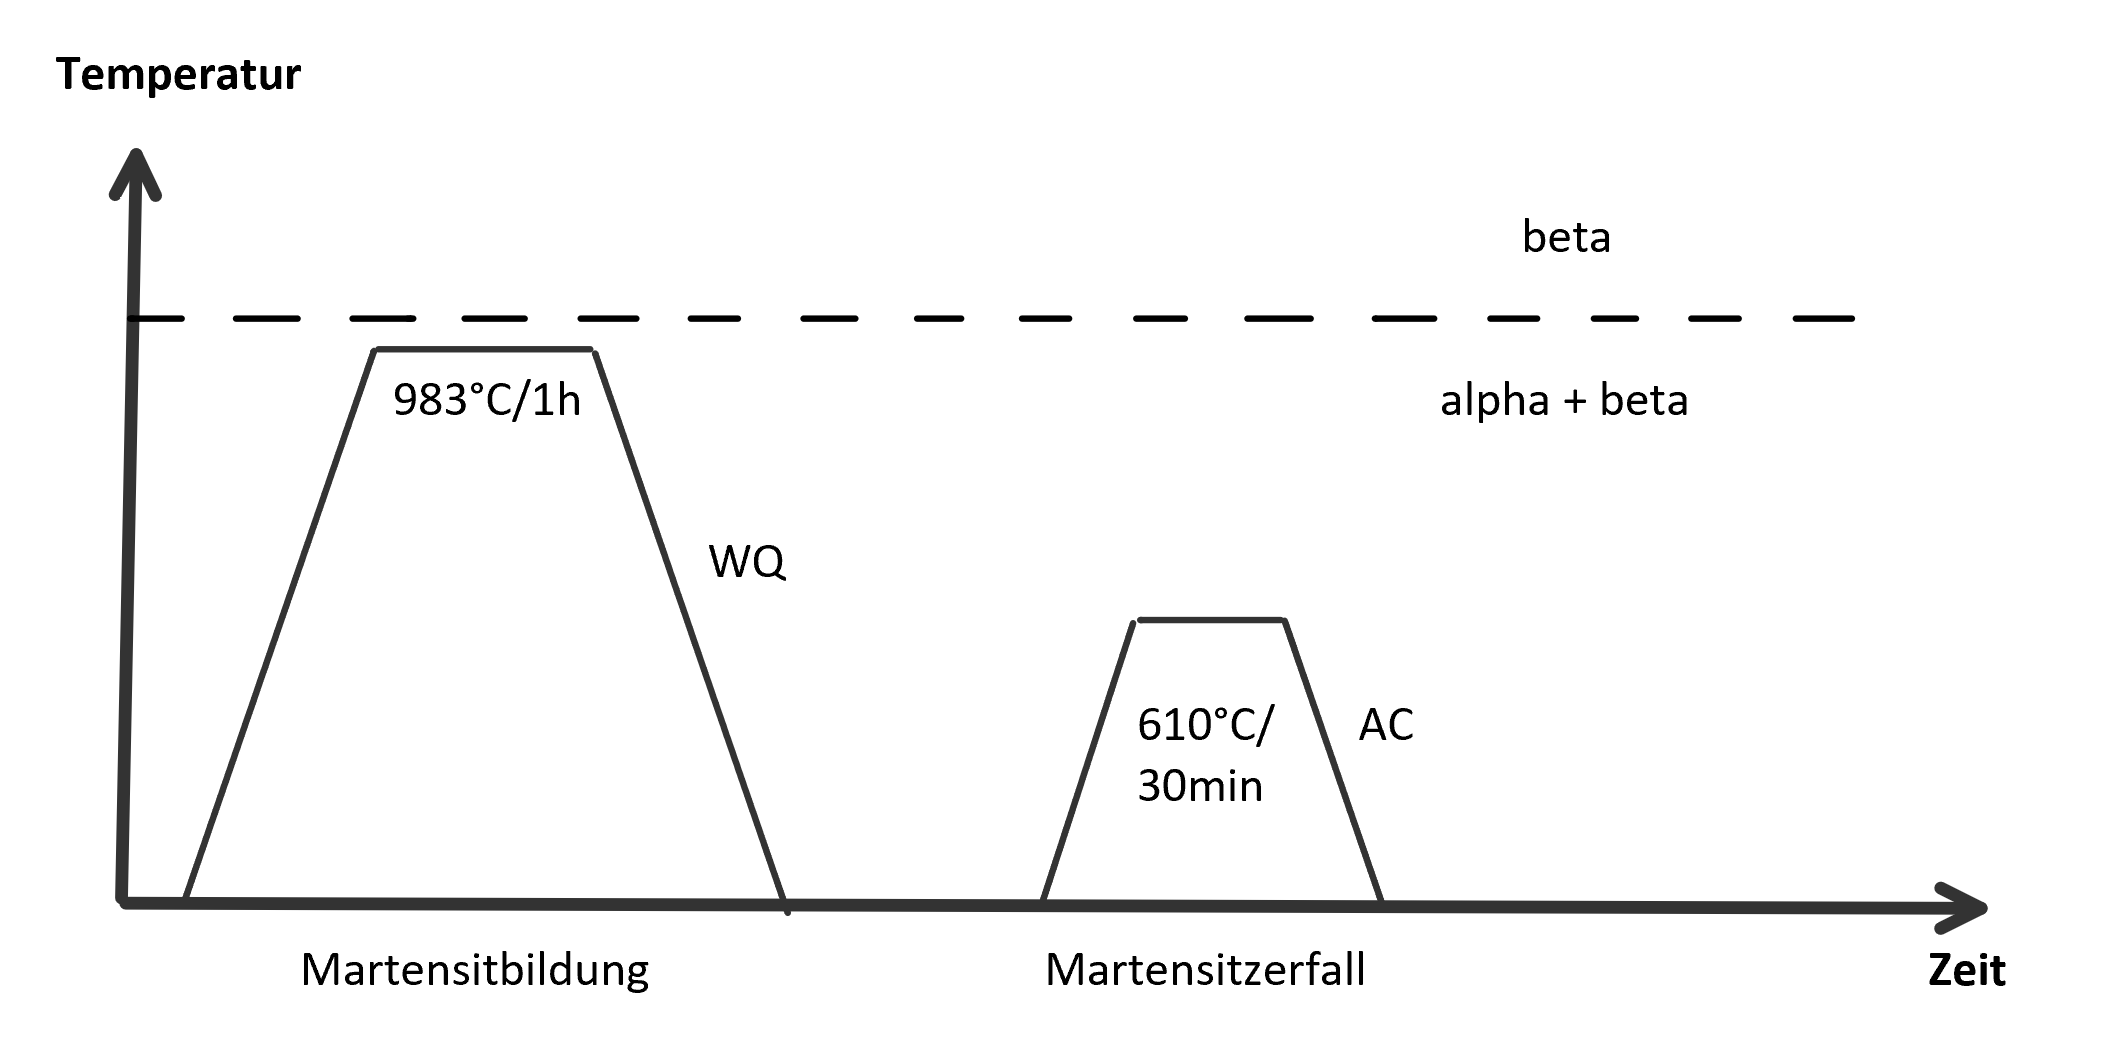
\includegraphics[width=0.9\textwidth]{./Bilder/SQ.png}}
	\caption{Wärmebehandlungsdiagramm von dem Solution Treatment and Quenching + aging}
	\label{fig:SQ}
\end{figure}

\section{Ergebnisse (PH)}

Die durch den ersten Behandlungschritt entstandene Mikrostruktur wurde unter dem Lichtmikroskop ausgewertet und ist in Abbildung \ref{fig:abbildung-19} aufgeführt.

\begin{figure}[h]
	\centering
	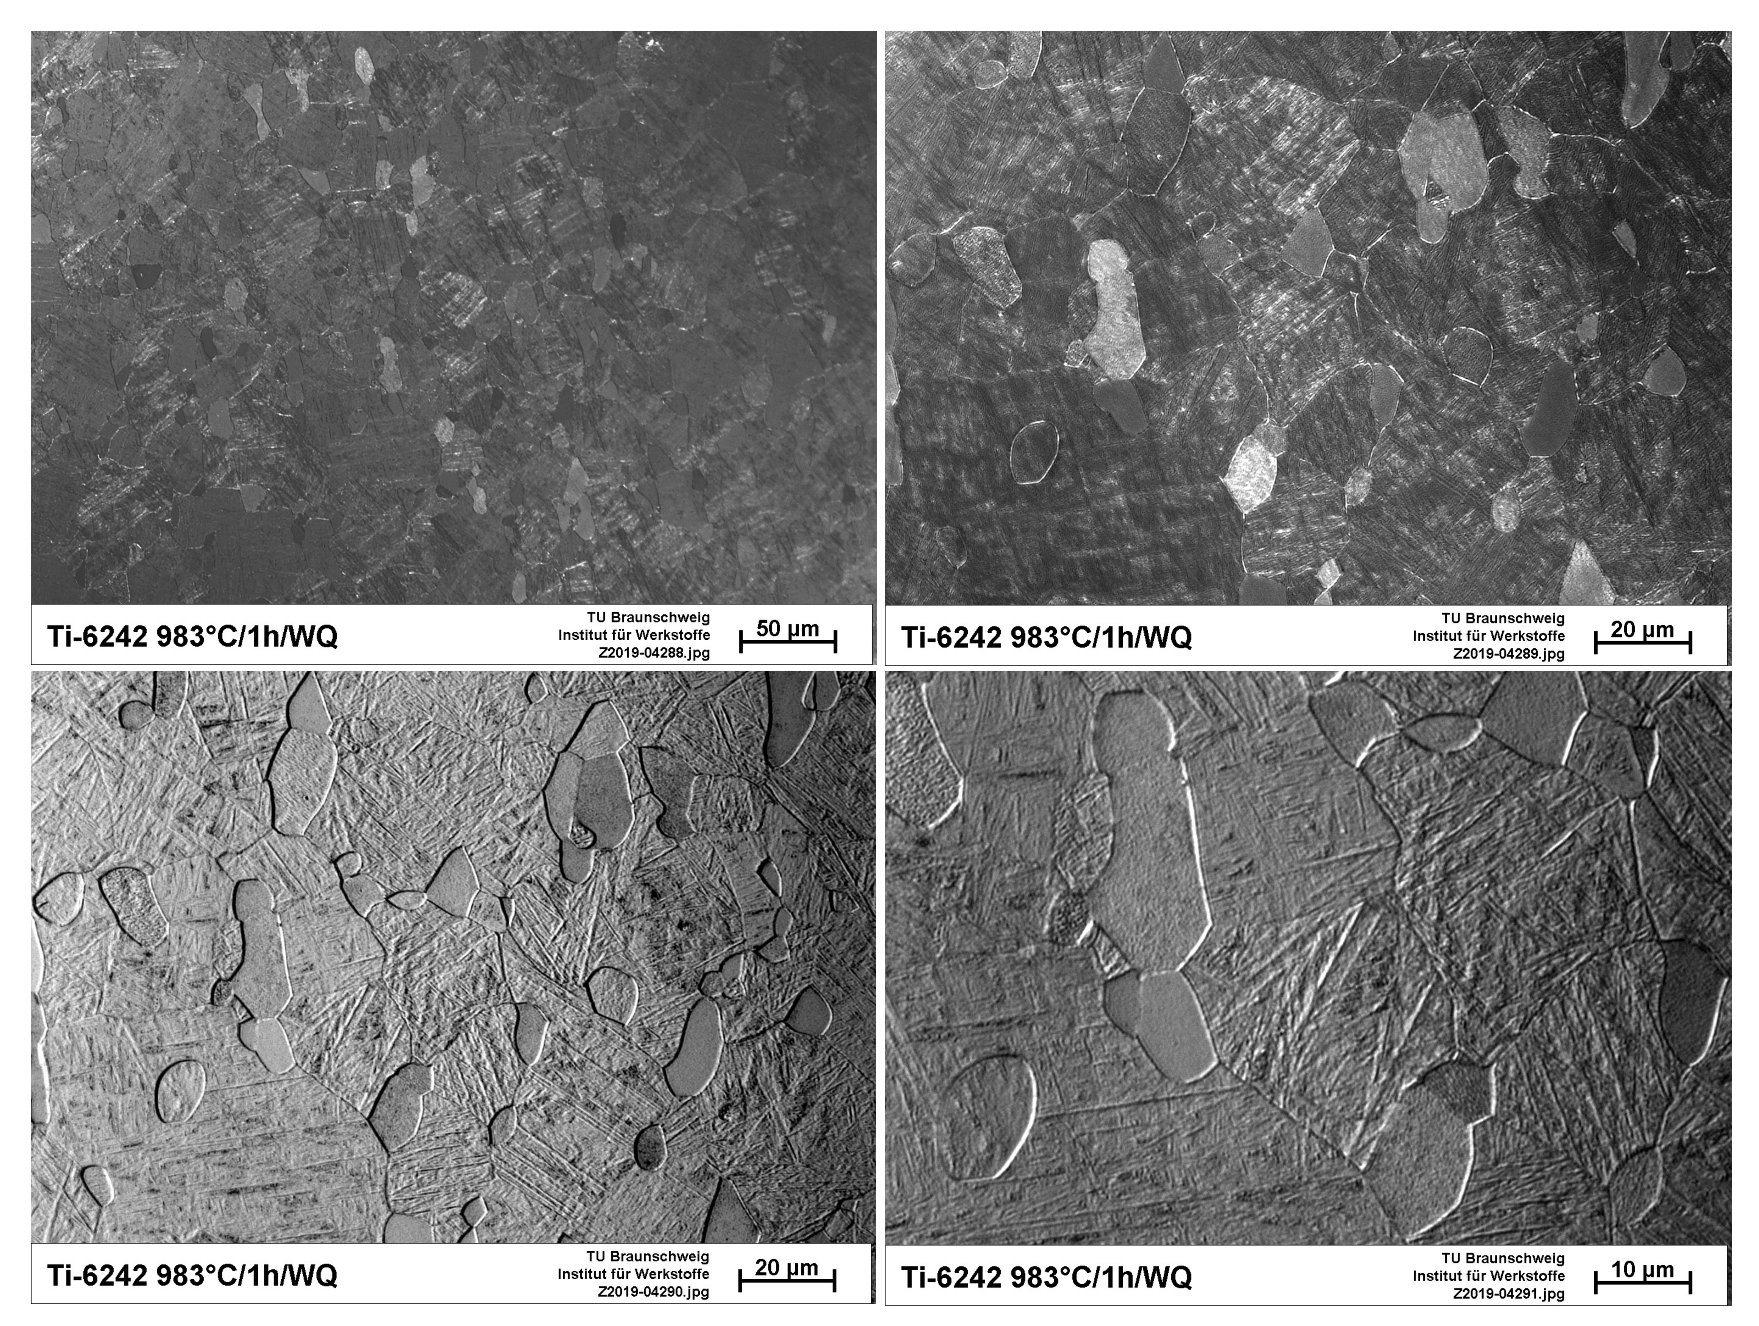
\includegraphics[width=1.0\linewidth]{./Bilder/Abbildung 19.png}
	\caption[Abbildung 19]{$\alpha_p$-$\alpha'$-Gefüge unter dem Lichtmikroskop bei verschiedenen Vergrößerungen (C-DIC)}
	\label{fig:abbildung-19}
\end{figure}

Die anschließende Härteprüfung ergab eine mittlere Vickershärte von 405 HV.

Die Auswertung des zweiten Wärmebehandlungsschritts unter dem REM ist in den Abbildungen \ref{fig:abbildung-26} und \ref{fig:abbildung-27} zusammengefasst.

\begin{figure}[h]
	\centering
	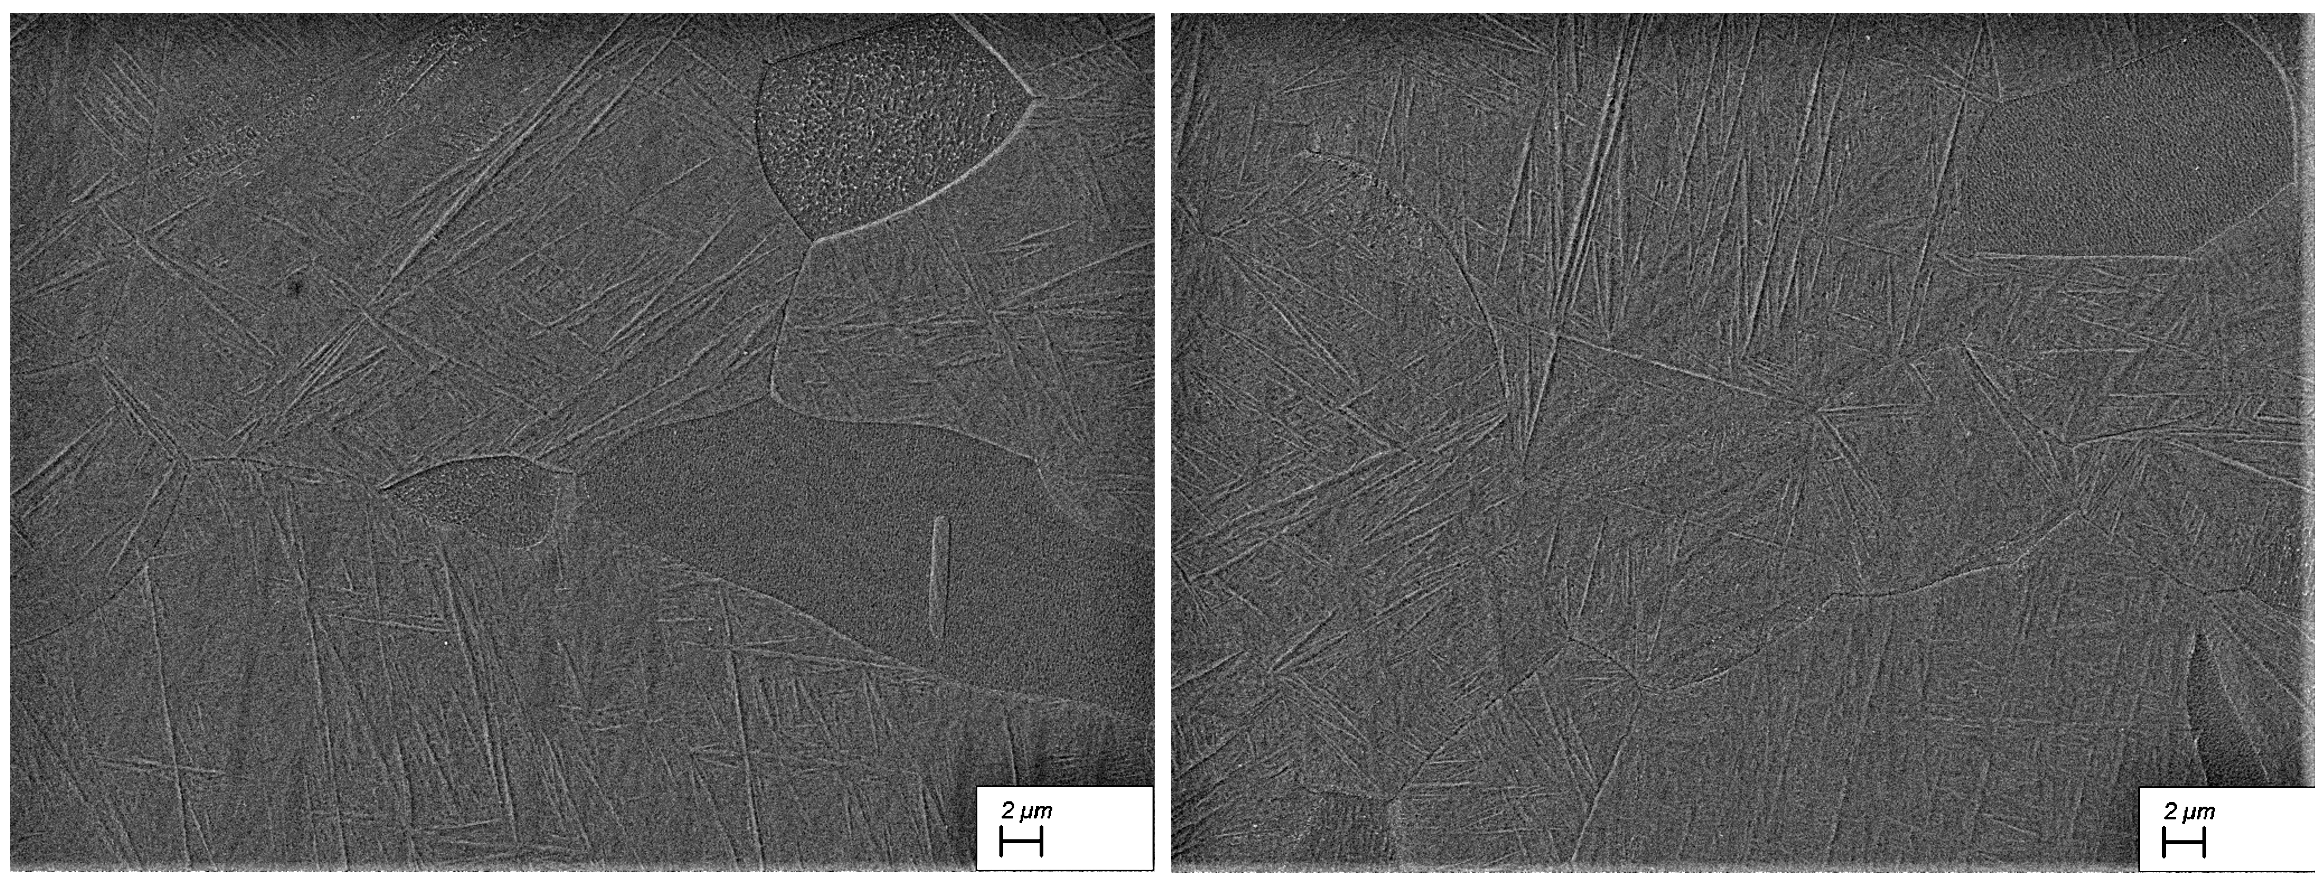
\includegraphics[width=1.0\linewidth]{./Bilder/Abbildung 26.png}
	\caption[Abbildung 26]{983$^\circ$C/1h/WQ + 610$^\circ$C/16min/AC, REM}
	\label{fig:abbildung-26}
\end{figure}

\begin{figure}[h]
	\centering
	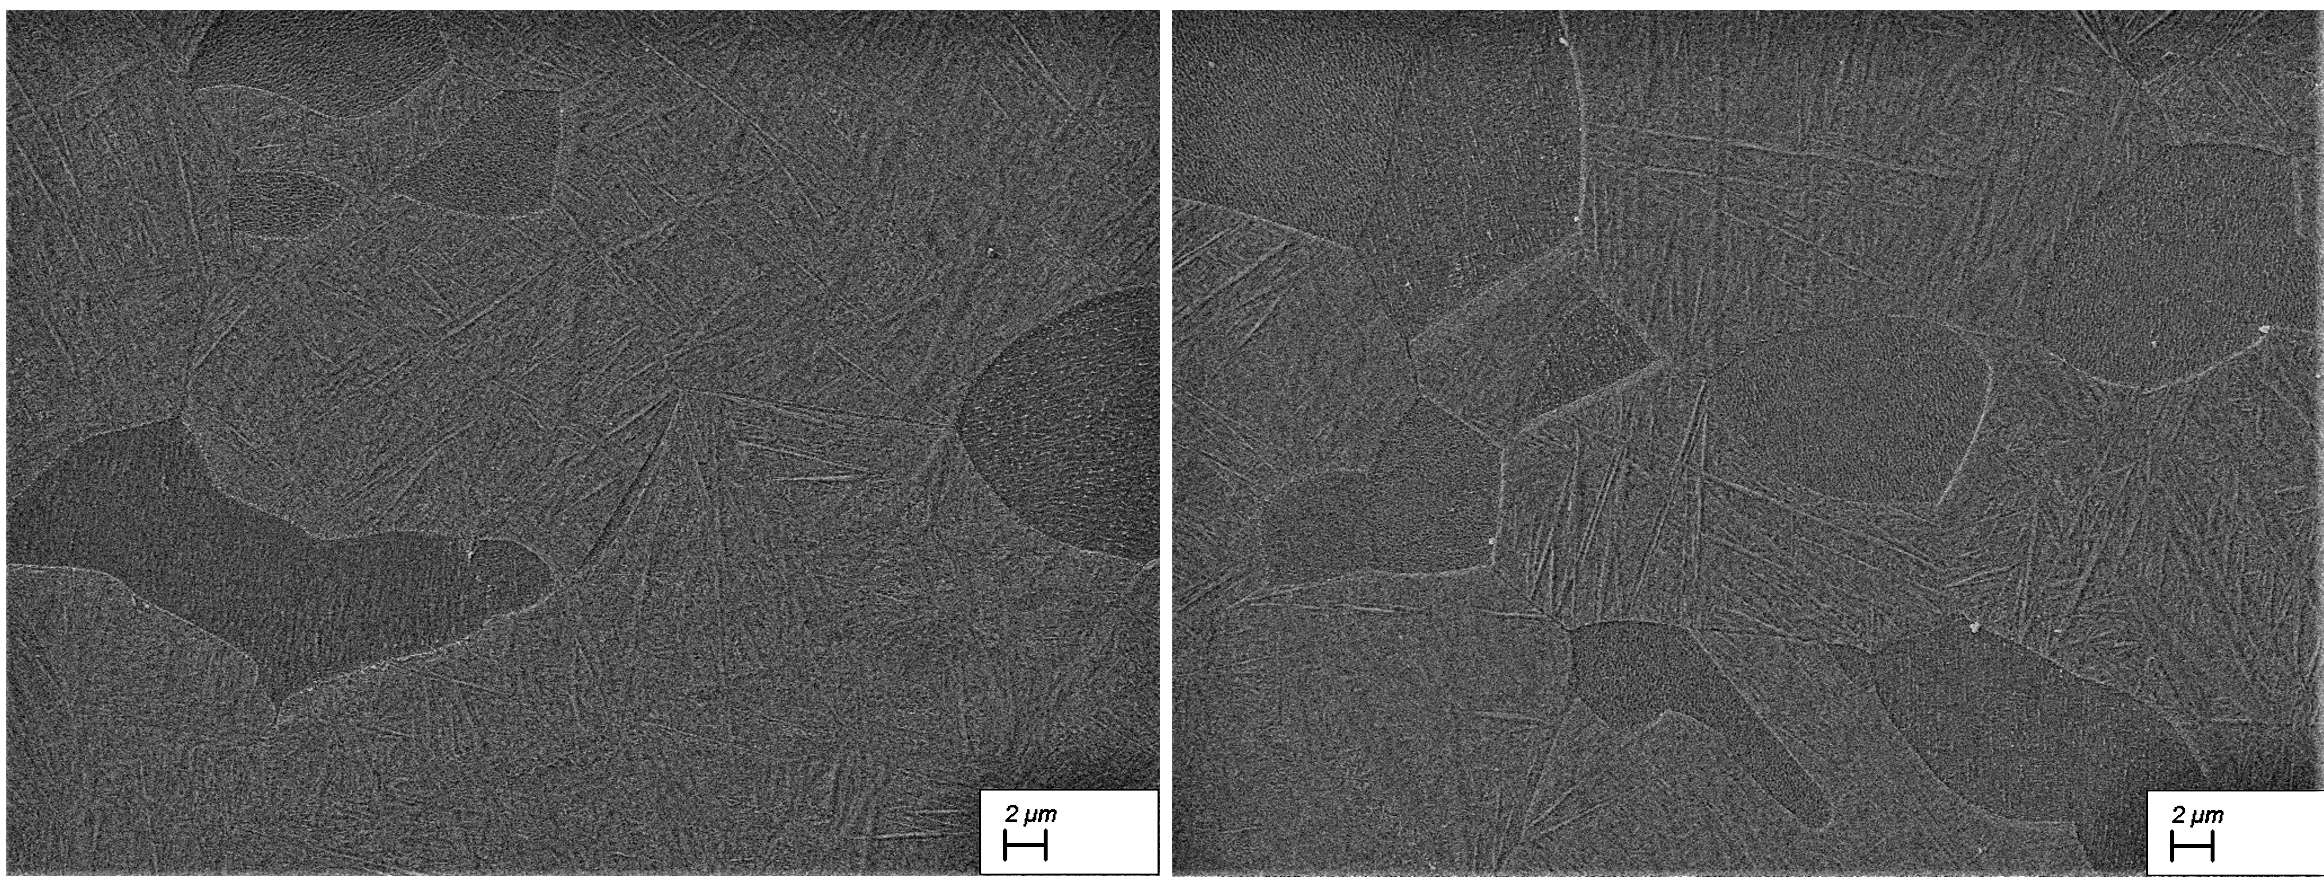
\includegraphics[width=1.0\linewidth]{./Bilder/Abbildung 27.png}
	\caption[Abbildung 27]{983$^\circ$C/1h/WQ + 610$^\circ$C/30min/AC, REM}
	\label{fig:abbildung-27}
\end{figure}

In den Abbildungen \ref{fig:abbildung-26} und \ref{fig:abbildung-27} ist zu erkennen, dass keine Veränderung in dem Gefüge im Vergleich zum vorherigen Schritt feststellbar ist. Es kann davon ausgegangen werden, dass der geplante Martensitzerfall nicht stattgefunden hat.

Die Ergebnisse der Härteprüfung nach diesem zweiten Schritt sind in Tabelle \ref{Tabelle 9} aufgeführt.

\begin{table}[h]
	\centering
	\begin{tabular}{|c|c|}
		\hline 
		Probe & Härte in HV \\ 
		\hline 
		983$^\circ$C/1h/WQ + 610$^\circ$C/16min/AC & 405 \\ 
		\hline 
		983$^\circ$C/1h/WQ + 610$^\circ$C/30min/AC & 400 \\ 
		\hline 
	\end{tabular} 
	\caption{Ergebnisse der Härteprüfung nach der zweiten Wärmebehandlung, $\alpha_p$- $\alpha'$ Gefüge}
	\label{Tabelle 9}
\end{table}

Es ist zu erkennen, dass auch die Härte unverändert im Vergleich zum vorherigen Schritt blieb.

\section{Diskussion (ZB)}

\paragraph{Glühen und Abschrecken}
Vor dem Abschrecken stellt sich ein zweiphasiges Gefüge ein ($\alpha$- und $\beta$-Phase). Der große $\beta$-Anteil des Gefüges konnte aber durch die Diffusion von 2\% Molybdän nicht stabilisiert werden und wandelte sich beim Abschrecken martensitisch um. Die Bildung von den Martensit-Nadeln verfeinert das Gefüge. Das hat dazu geführt, dass sich die Härte dieser Proben von 331 auf 405 HV gestiegen ist. 

\paragraph{Anlassen} Nach dem Anlassen hat sich gezeigt, dass $\alpha'$ nicht zerfallen konnte. Das ist wahrscheinlich darauf zurückzuführen, dass die Haltezeit von 30 min nicht ausreichend für die Umwandlung der Martensitnadeln in  $\beta$ + $\alpha$ war. Eine weitere Erklärung dafür könnte sein, dass diese Transformation bei 610$^\circ$C so langsam ablief, dass sie innerhalb von 30 min nicht stattfinden konnte.
Deshalb waren keine Gefüge- oder Härteänderungen im Vergleich zu dem ersten Schritt festzustellen. 


\chapter{Zugversuche }

\section{Durchführung (ZB)}

Um die Einflüsse der Wärmebehandlungen genauer betrachten zu können, wurden weitere wichtige mechanische Kennwerte wie die Duktilität, Zugfestigkeit und Bruchdehnung von 8 Proben durch Zugversuche ermittelt. \\
Um auch den Einfluss von dem Martensitzerfall in der ersten Strategie auf die Duktilität genauer diskutieren zu können, werden auch die Proben 7 und 8 untersucht. Eine Übersicht über die für den Zugversuch ausgewählten Proben ist in Tabelle \ref{tab:ubersicht} aufgeführt.


\begin{table}[h]
	\centering
	\begin{tabular}{|c|c|}
		\hline 
		Probe & Wärmebehandlung \\ 
		\hline 
		1 & AR1 \\ 
		\hline 
		2 & AR2 \\ 
		\hline 
		3 &  983$^\circ$C/1h/AC + 950$^\circ$C/16min/WQ + 610$^\circ$C/16min/AC \\ 
		\hline 
		4 &  983$^\circ$C/1h/AC + 950$^\circ$C/16min/WQ + 610$^\circ$C/16min/AC \\ 
		\hline 
		5 &  983$^\circ$C/1h/WQ + 610$^\circ$C/30min/AC \\ 
		\hline 
		6 &  983$^\circ$C/1h/WQ + 610$^\circ$C/30min/AC \\ 
		\hline 
		7 &  983$^\circ$C/1h/AC + 950$^\circ$C/16min/WQ \\ 
		\hline 
		8 &  983$^\circ$C/1h/AC + 950$^\circ$C/16min/WQ \\ 
		\hline 
	\end{tabular}
    \caption{Übersicht der gewählten Proben für den Zugversuch}
	\label{tab:ubersicht} 
\end{table}

\section{Ergebnisse (VR)}

Die gesamten Ergebnisse der Zugversuche sind in Tabelle \ref{tab:zugversuche} zusammengefasst. Es ist eine Zugfestigkeitssteigerung bei allen Wärmebehandlungen gegenüber den AR-Proben zu erkennen. Die TS-STDA hat eine Steigerung der Zugfestigkeit von 7,6\% mit Martensitzerfall, 4,3\% ohne Martensitzerfall und die Strategie 2 1,3\%  gebracht. Die Bruchdehnung ist jedoch bei allen wärmebehandelten Proben unter die geforderten 10\% gefallen. 
Wie in Abbildung \ref{fig:zugkaputt} zu sehen ist, sind alle Proben am Rand des parallelen Fließbereichs der Zugprobe eingeschnürt und gebrochen. Dies hat zur Folge das nicht die gesamte Dehnung der Probe von den Wegaufnehmern aufgenommen wurde und die tatsächliche Dehnung der Proben wahrscheinlich höher ist als gemessen. In den Spannungs-Dehnungs-Diagrammen in den Abb. \ref{fig:vergleich-vor-und-nach-zerfall}--\ref{fig:vergleich-alle-proben} ist eine Hysteresekurve im Bereich von 1\% Dehnung zu sehen. Sie wird automatisch vom Steuerungsprogramm der Zugmaschine durchgeführt, um Abweichungen im elastischen Werkstoffverhalten zwischen Be- und Entlastung aufzunehmen. 


\begin{figure}
	\centering
	\includegraphics[width=0.6\linewidth]{./Bilder/Zugproben_kaputt}
	\caption{links: $\alpha_p + \alpha^\prime$-Probe, mitte und rechts: TS-STDA}
	\label{fig:zugkaputt}
\end{figure}

\begin{figure}
	\centering
	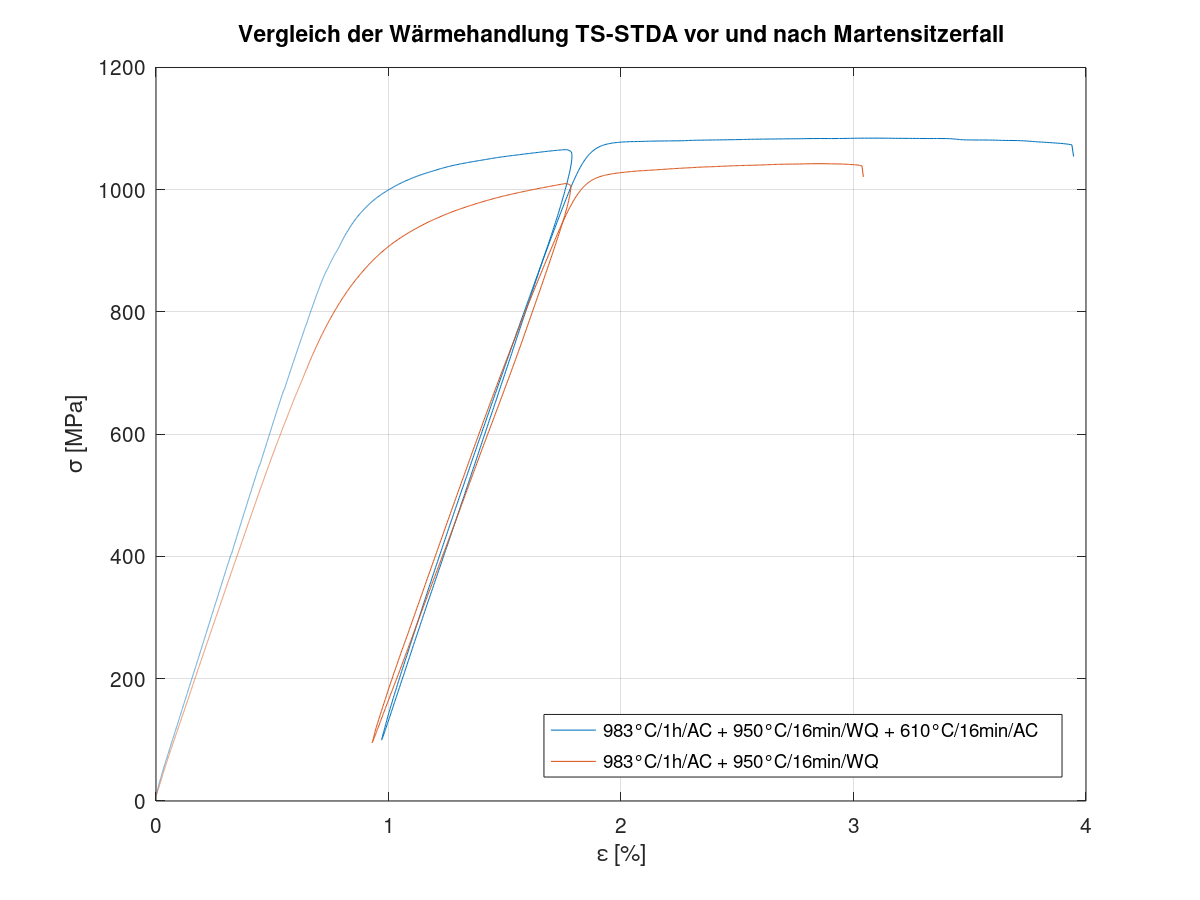
\includegraphics[width=0.8\linewidth]{./Bilder/Vergleich vor und nach Zerfall}
	\caption{Spannungs-Dehnungs-Diagramm für TS-STDA vor und nach dem Martensitzerfall}
	\label{fig:vergleich-vor-und-nach-zerfall}
\end{figure}

\begin{figure}
	\centering
	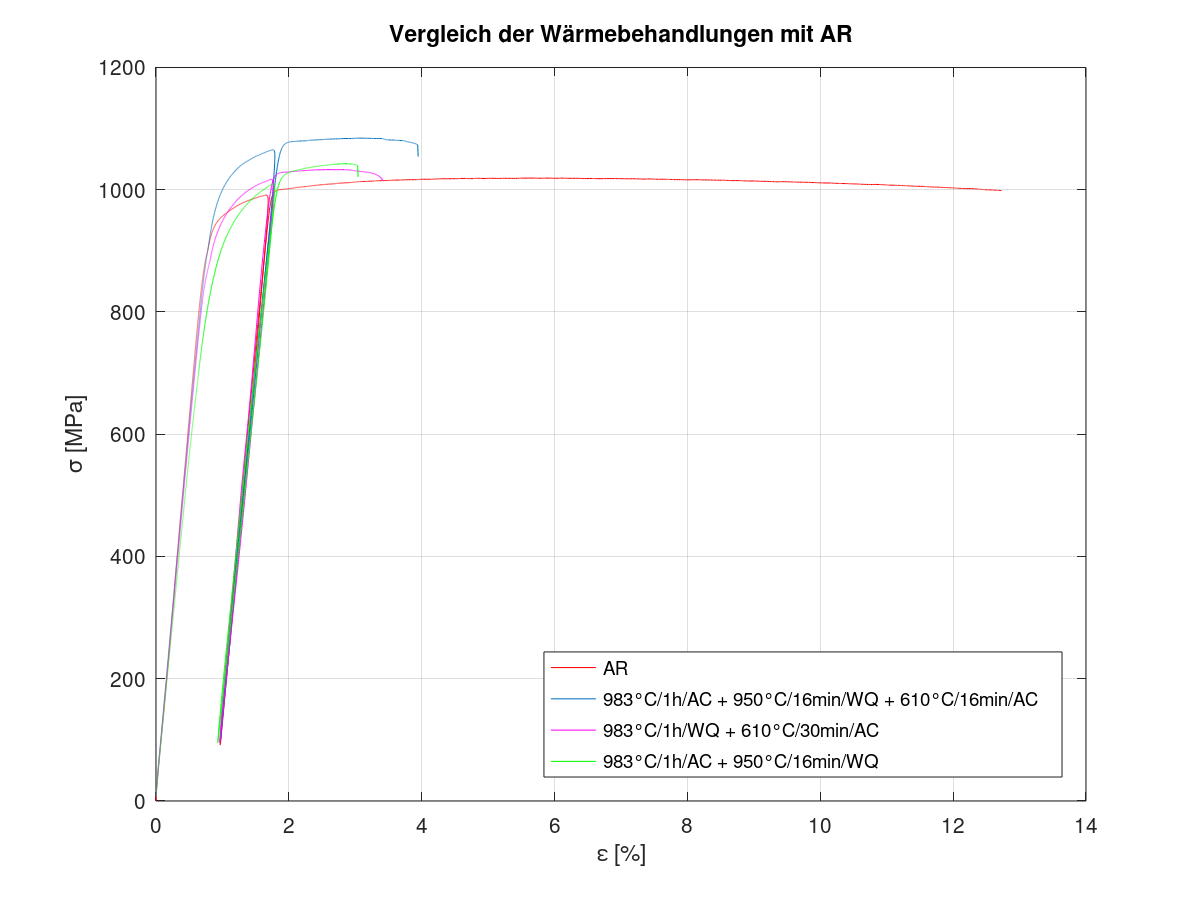
\includegraphics[width=0.8\linewidth]{./Bilder/Vergleich aller Proben}
	\caption{Spannungs-Dehnungs-Diagramm für alle Proben}
	\label{fig:vergleich-alle-proben}
\end{figure}

\begin{table}
	\centering
	\begin{tabular}{|c|c|c|c|c|c|c|c|}
		\hline
		Probe & $d_0$ [mm] & $S_0$ [mm$^2$] & \textit{E} [GPa] & $R_{p0,2}$ [MPa]& $R_m$ [MPa]& $A_g$ [\%]& $A$ [\%]\\
		\hline
		1 & 5,06 & 20,11 & 128 & 956 & 1019&4,8&17,9 \\
		\hline
		2 &5,04&19,95&122&946&1013&5,1&15,7\\
		\hline
		3 & 5,11&20,51& 122&1015&1085&2,1&3,0\\
		\hline
		4 &5,16& 20,91& 117 & 1007& 1090& 1,7&  1,9 \\
		\hline
		5&5,04 &19,95& 120& 952& 1033& 1,9 &2,5\\
		\hline
		6 &5,02& 19,79& 124& 968& 1023 &1,0 & 2,0\\
		\hline
		7&5,17& 20,99& 113& 925& 1042& 1,9& 2,1\\
		\hline
		8 & 5,12 & 20,59 & 118 & 952 & 1063 & 1,3 & 1,4\\
		\hline
	\end{tabular}
	\caption{Messwerte der Zugversuche bei 23,3$^\circ$C Raumtemperatur}
	\label{tab:zugversuche}
	
\end{table}

\pagebreak

\section{Diskussion der Ergebnisse (ZB)}

AR-Proben haben ein globulares Gefüge mit $\alpha$- und transformierter $\beta$-Phase (Abbildung \ref{fig:abbildung-8} a). Durch den großen Anteil an $\alpha_p$ konnten sich sehr feine $\alpha$-Lamellen in der transformierten $\beta$-Phase bilden, die für eine Duktilitätssteigerung sorgen. Aufgrund dieser feinen Strukturen haben AR-Proben eine relativ hohe Bruchdehnung \cite{Lutjering.2007}.

Die Proben 7 und 8 haben durch das Duplex-Glühen neben Martensit und kleinen $\alpha_p$-Körnern feine $\alpha$-Lamellen. Außerdem haben die Proben 5--8 im Vergleich zu den AR-Proben durch die Bildung von dünnen Martensitplatten feinere Gefügestrukturen. Dies führte vermutlich bei diesen Proben zu der Festigkeitszunahme. Das erklärt auch, dass Martensit, der nur eine beschränkte Duktiliät besitzt \cite{Lutjering.2007}, zu der niedrigen Duktilität dieser Proben geführt hat.\\
Des Weiteren hat die Probe 3 eine höhere Duktilität und Festigkeit gegenüber den Proben 7 und 8. Das kann durch den partiellen Martensit-Zerfall bzw. die Teiltransformation von $\alpha'$ in $\alpha$- und $\beta$-Phasen im letzten Schritt der Strategie 1 erklärt werden. Die Verfeinerung des Gefüges durch eine partielle Dekomposition der Martensitnadeln führt einerseits zu einer Steigerung der  Zugfestigkeit  und gleichzeitig zu einer Zunahme der Duktilität. 
Das bedeutet, dass ein weiterer Zerfall der Martensitstrukturen bei beiden Strategien zu einer Verbesserung der Bruchdehnung führen könnte. Dabei soll sich eine gröbere Gefügestruktur durch die Transformation von Martensit vollständig in $\alpha$- und $\beta$-Körner bilden. Dies ist möglich, wenn Proben aus Strategie 1 und 2 beim letzten Anlassen für längere Zeit bzw. bei höheren Temperaturen geglüht werden. Ein Beispiel für diese Optimierung der beiden Strategien zeigt die Tabelle \ref{wBZ}.



\begin{table}[h]
	\centering
	\begin{tabular}{|c|c|}
		\hline 
		Strategie & Wärmebehandlung \\ 
		\hline 
		1 & 983$^\circ$C/1h/AC + 950$^\circ$C/16$\pm $4min/WQ + 610$^\circ$C/1h/AC\\ 
		\hline 
		2 &  983$^\circ$C/1h/WQ + 800$^\circ$C/1.5--2h/AC \\ 
		\hline 
	\end{tabular} 
	\caption{Optimierungsbeispiele für Strategie 1 und 2}
	\label{wBZ}
	
	
\end{table}

Durch beide Strategien konnte eine Verfestigung von Ti-6242 erreicht werden. Die Dehngrenze hat dabei  die 10\% unterschritten. 
Aufgrund der kurzen Anlasszeiten und des starken Einflusses der Glühtemperatur auf die Gefügestruktur, ist die Reproduzierbarkeit der ersten Strategie für die Industrie ungenügend.















\chapter{Fazit und Ausblick}

tbd

\chapter*{Eidesstattliche Erkl"arung}\label{s:eid_erkl}


Hiermit erklären wir, Ziad Ben Hadj Salem, Thiago Coelho Jordao, Patrick Hartmann und Viktor Rein des Eides statt, die vorliegende Projektarbeit selbstständig und ohne
fremde Hilfe verfasst und keine anderen als die angegebenen Hilfsmittel verwendet zu
haben.

\vspace*{3cm}
Braunschweig, Datum

%%only blank page
\newpage
\thispagestyle{empty}
\mbox{}


% Literaturverzeichnis
\newpage
\bibliographystyle{unsrt}
\bibliography{Literatur}		% Pfad zur *.bib-Datei
\addcontentsline{toc}{chapter}{Literatur}
%\printbibliography


\end{document}